\documentclass[]{book}
\usepackage{lmodern}
\usepackage{amssymb,amsmath}
\usepackage{ifxetex,ifluatex}
\usepackage{fixltx2e} % provides \textsubscript
\ifnum 0\ifxetex 1\fi\ifluatex 1\fi=0 % if pdftex
  \usepackage[T1]{fontenc}
  \usepackage[utf8]{inputenc}
\else % if luatex or xelatex
  \ifxetex
    \usepackage{mathspec}
  \else
    \usepackage{fontspec}
  \fi
  \defaultfontfeatures{Ligatures=TeX,Scale=MatchLowercase}
\fi
% use upquote if available, for straight quotes in verbatim environments
\IfFileExists{upquote.sty}{\usepackage{upquote}}{}
% use microtype if available
\IfFileExists{microtype.sty}{%
\usepackage{microtype}
\UseMicrotypeSet[protrusion]{basicmath} % disable protrusion for tt fonts
}{}
\usepackage{hyperref}
\hypersetup{unicode=true,
            pdftitle={Data cleaning guide for the Rotterdam Study},
            pdfauthor={Paloma Rojas Saunero, Eline Vinke},
            pdfborder={0 0 0},
            breaklinks=true}
\urlstyle{same}  % don't use monospace font for urls
\usepackage{color}
\usepackage{fancyvrb}
\newcommand{\VerbBar}{|}
\newcommand{\VERB}{\Verb[commandchars=\\\{\}]}
\DefineVerbatimEnvironment{Highlighting}{Verbatim}{commandchars=\\\{\}}
% Add ',fontsize=\small' for more characters per line
\usepackage{framed}
\definecolor{shadecolor}{RGB}{248,248,248}
\newenvironment{Shaded}{\begin{snugshade}}{\end{snugshade}}
\newcommand{\AlertTok}[1]{\textcolor[rgb]{0.94,0.16,0.16}{#1}}
\newcommand{\AnnotationTok}[1]{\textcolor[rgb]{0.56,0.35,0.01}{\textbf{\textit{#1}}}}
\newcommand{\AttributeTok}[1]{\textcolor[rgb]{0.77,0.63,0.00}{#1}}
\newcommand{\BaseNTok}[1]{\textcolor[rgb]{0.00,0.00,0.81}{#1}}
\newcommand{\BuiltInTok}[1]{#1}
\newcommand{\CharTok}[1]{\textcolor[rgb]{0.31,0.60,0.02}{#1}}
\newcommand{\CommentTok}[1]{\textcolor[rgb]{0.56,0.35,0.01}{\textit{#1}}}
\newcommand{\CommentVarTok}[1]{\textcolor[rgb]{0.56,0.35,0.01}{\textbf{\textit{#1}}}}
\newcommand{\ConstantTok}[1]{\textcolor[rgb]{0.00,0.00,0.00}{#1}}
\newcommand{\ControlFlowTok}[1]{\textcolor[rgb]{0.13,0.29,0.53}{\textbf{#1}}}
\newcommand{\DataTypeTok}[1]{\textcolor[rgb]{0.13,0.29,0.53}{#1}}
\newcommand{\DecValTok}[1]{\textcolor[rgb]{0.00,0.00,0.81}{#1}}
\newcommand{\DocumentationTok}[1]{\textcolor[rgb]{0.56,0.35,0.01}{\textbf{\textit{#1}}}}
\newcommand{\ErrorTok}[1]{\textcolor[rgb]{0.64,0.00,0.00}{\textbf{#1}}}
\newcommand{\ExtensionTok}[1]{#1}
\newcommand{\FloatTok}[1]{\textcolor[rgb]{0.00,0.00,0.81}{#1}}
\newcommand{\FunctionTok}[1]{\textcolor[rgb]{0.00,0.00,0.00}{#1}}
\newcommand{\ImportTok}[1]{#1}
\newcommand{\InformationTok}[1]{\textcolor[rgb]{0.56,0.35,0.01}{\textbf{\textit{#1}}}}
\newcommand{\KeywordTok}[1]{\textcolor[rgb]{0.13,0.29,0.53}{\textbf{#1}}}
\newcommand{\NormalTok}[1]{#1}
\newcommand{\OperatorTok}[1]{\textcolor[rgb]{0.81,0.36,0.00}{\textbf{#1}}}
\newcommand{\OtherTok}[1]{\textcolor[rgb]{0.56,0.35,0.01}{#1}}
\newcommand{\PreprocessorTok}[1]{\textcolor[rgb]{0.56,0.35,0.01}{\textit{#1}}}
\newcommand{\RegionMarkerTok}[1]{#1}
\newcommand{\SpecialCharTok}[1]{\textcolor[rgb]{0.00,0.00,0.00}{#1}}
\newcommand{\SpecialStringTok}[1]{\textcolor[rgb]{0.31,0.60,0.02}{#1}}
\newcommand{\StringTok}[1]{\textcolor[rgb]{0.31,0.60,0.02}{#1}}
\newcommand{\VariableTok}[1]{\textcolor[rgb]{0.00,0.00,0.00}{#1}}
\newcommand{\VerbatimStringTok}[1]{\textcolor[rgb]{0.31,0.60,0.02}{#1}}
\newcommand{\WarningTok}[1]{\textcolor[rgb]{0.56,0.35,0.01}{\textbf{\textit{#1}}}}
\usepackage{longtable,booktabs}
\usepackage{graphicx,grffile}
\makeatletter
\def\maxwidth{\ifdim\Gin@nat@width>\linewidth\linewidth\else\Gin@nat@width\fi}
\def\maxheight{\ifdim\Gin@nat@height>\textheight\textheight\else\Gin@nat@height\fi}
\makeatother
% Scale images if necessary, so that they will not overflow the page
% margins by default, and it is still possible to overwrite the defaults
% using explicit options in \includegraphics[width, height, ...]{}
\setkeys{Gin}{width=\maxwidth,height=\maxheight,keepaspectratio}
\IfFileExists{parskip.sty}{%
\usepackage{parskip}
}{% else
\setlength{\parindent}{0pt}
\setlength{\parskip}{6pt plus 2pt minus 1pt}
}
\setlength{\emergencystretch}{3em}  % prevent overfull lines
\providecommand{\tightlist}{%
  \setlength{\itemsep}{0pt}\setlength{\parskip}{0pt}}
\setcounter{secnumdepth}{5}
% Redefines (sub)paragraphs to behave more like sections
\ifx\paragraph\undefined\else
\let\oldparagraph\paragraph
\renewcommand{\paragraph}[1]{\oldparagraph{#1}\mbox{}}
\fi
\ifx\subparagraph\undefined\else
\let\oldsubparagraph\subparagraph
\renewcommand{\subparagraph}[1]{\oldsubparagraph{#1}\mbox{}}
\fi

%%% Use protect on footnotes to avoid problems with footnotes in titles
\let\rmarkdownfootnote\footnote%
\def\footnote{\protect\rmarkdownfootnote}

%%% Change title format to be more compact
\usepackage{titling}

% Create subtitle command for use in maketitle
\providecommand{\subtitle}[1]{
  \posttitle{
    \begin{center}\large#1\end{center}
    }
}

\setlength{\droptitle}{-2em}

  \title{Data cleaning guide for the Rotterdam Study}
    \pretitle{\vspace{\droptitle}\centering\huge}
  \posttitle{\par}
    \author{Paloma Rojas Saunero, Eline Vinke}
    \preauthor{\centering\large\emph}
  \postauthor{\par}
      \predate{\centering\large\emph}
  \postdate{\par}
    \date{2019-10-15}

\usepackage{booktabs}

\begin{document}
\maketitle

{
\setcounter{tocdepth}{1}
\tableofcontents
}
\hypertarget{about}{%
\chapter{About}\label{about}}

Data cleaning (wrangling) will be the first to face after obtaining the raw data for your research.

To facilitate this process, we want to provide a guide that describes how to approach the raw data from the Rotterdam study and provides the corresponding code to approach each variable. The intention is that all students becoming familiar with the data and develop the essencial skills for a reproducible data cleaning.

We will use the \textbf{tidyverse} language and ecosystem. If you are not familiar with the tidyverse and the pipe operator \textbf{\%\textgreater\%} you will want to read \href{https://r4ds.had.co.nz/pipes.html}{this book}. This book contains a description of the essencial tidyverse tools.

\textbf{Note:} If you find any bug, typo, have suggestions, questions or you want to include a chapter in this guide please get in contact with us! We want to make this as collaborative as possible.

Paloma: \href{mailto:l.rojassaunero@erasmusmc.nl}{\nolinkurl{l.rojassaunero@erasmusmc.nl}}

Eline: \href{mailto:e.vinke@erasmusmc.nl}{\nolinkurl{e.vinke@erasmusmc.nl}}

Github repository: \url{https://github.com/palolili23/cov_rs}

\hypertarget{intro}{%
\chapter{Introduction}\label{intro}}

\hypertarget{prerequisites}{%
\section{Prerequisites}\label{prerequisites}}

\begin{itemize}
\item
  Install R and Rstudio IDE
\item
  Install and open the following packages: \texttt{tidyverse}, \texttt{rio}, \texttt{here}.
\item
  Create an R project with a folder for your raw data (We will name this folder \texttt{00\_raw\_data})
\item
  Data can be accessed from the following: \href{https://epi-wiki.erasmusmc.nl/wiki/ergowiki/index.php/Ergobasics}{link}
\end{itemize}

\hypertarget{rotterdam-study-data-structure}{%
\section{Rotterdam study data structure}\label{rotterdam-study-data-structure}}

We followed the structure of the visit process to name the cohorts and visits:

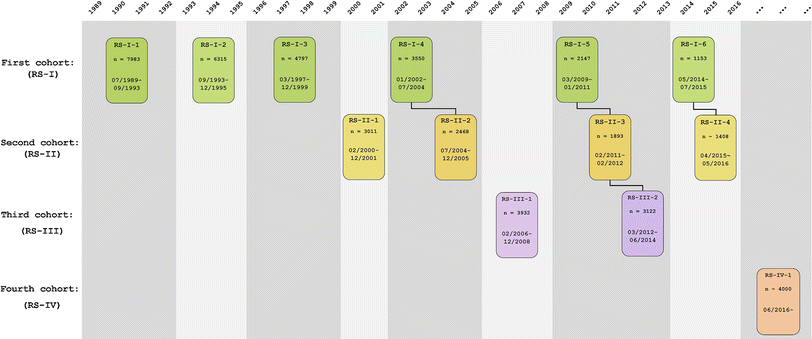
\includegraphics[width=1\linewidth]{./rs}

In the following structure:

\begin{tabular}{l|l|l|l|l|l}
\hline
var1 & var2 & var3 & var4 & var5 & var6\\
\hline
RS-I-1 & RS-I-2 & RS-I-3 & RS-I-4 & RS-I-5 & RS-I-6\\
\hline
NA & NA & RS-II-1 (ep) & RS-II-2 & RS-II-3 & RS-II-4\\
\hline
NA & NA & NA & RS-III-1 (ej) & RS-III-2 & RS-III-3\\
\hline
\end{tabular}

We name each variable in the same way over the waves and end with the number that corresponds to the visit.

\hypertarget{overview-of-the-process-to-clean-a-variable}{%
\section{Overview of the process to clean a variable}\label{overview-of-the-process-to-clean-a-variable}}

Each small chapter will provide the code to clean each of the variables that are oftenly used as covariates in any data analysis.

Since the name of the variables could have changed in each visit, and data is arranged in different ways, we decided to create a systematic flow of how the cleaning process is one covariate at a time, for all visits, for all cohorts.

The usuals steps will include:

\begin{enumerate}
\def\labelenumi{\arabic{enumi}.}
\tightlist
\item
  Import datasets for all the visits, for all cohorts.
\end{enumerate}

\begin{itemize}
\item
  Note that we use the \texttt{here} package to specify the folder/subfolder and file we want to import. We do this to avoid specifying the directory. This practice helps the reproducibility of the code as mentioned in the following \href{https://www.tidyverse.org/articles/2017/12/workflow-vs-script/}{link}

  \begin{itemize}
  \tightlist
  \item
    We will always include the subfix representing the cohort and visit. For example:
  \end{itemize}
\end{itemize}

\begin{Shaded}
\begin{Highlighting}[]
\NormalTok{rs1_}\DecValTok{1}\NormalTok{ <-}\StringTok{ }\KeywordTok{read_sav}\NormalTok{(here}\OperatorTok{::}\KeywordTok{here}\NormalTok{(}\StringTok{"00_raw_data"}\NormalTok{, }\StringTok{"visits"}\NormalTok{, }\StringTok{"Ergo1ResponseDetail_(22-jan-2015)_excerpt.sav"}\NormalTok{))}
\NormalTok{rs1_}\DecValTok{2}\NormalTok{ <-}\StringTok{ }\KeywordTok{read_sav}\NormalTok{(here}\OperatorTok{::}\KeywordTok{here}\NormalTok{(}\StringTok{"00_raw_data"}\NormalTok{, }\StringTok{"visits"}\NormalTok{, }\StringTok{"Ergo2ResponseDetail_(22-jan-2015)_excerpt.sav"}\NormalTok{))}
\NormalTok{rs1_}\DecValTok{3}\NormalTok{ <-}\StringTok{ }\KeywordTok{read_sav}\NormalTok{(here}\OperatorTok{::}\KeywordTok{here}\NormalTok{(}\StringTok{"00_raw_data"}\NormalTok{, }\StringTok{"visits"}\NormalTok{, }\StringTok{"e3_(3)_RESPONS_(22-feb-2016)_excerpt.sav"}\NormalTok{))}
\NormalTok{rs1_}\DecValTok{4}\NormalTok{ <-}\StringTok{ }\KeywordTok{read_sav}\NormalTok{(here}\OperatorTok{::}\KeywordTok{here}\NormalTok{(}\StringTok{"00_raw_data"}\NormalTok{, }\StringTok{"visits"}\NormalTok{, }\StringTok{"e4_(4)_RESPONS_(12-mar-2018)_excerpt.sav"}\NormalTok{))}
\NormalTok{rs1_}\DecValTok{5}\NormalTok{ <-}\StringTok{ }\KeywordTok{read_sav}\NormalTok{(here}\OperatorTok{::}\KeywordTok{here}\NormalTok{(}\StringTok{"00_raw_data"}\NormalTok{, }\StringTok{"visits"}\NormalTok{, }\StringTok{"e5_(5)_RESPONS_(22-jun-2016)_excerpt.sav"}\NormalTok{))}
\NormalTok{rs1_}\DecValTok{6}\NormalTok{ <-}\StringTok{ }\KeywordTok{read_sav}\NormalTok{(here}\OperatorTok{::}\KeywordTok{here}\NormalTok{(}\StringTok{"00_raw_data"}\NormalTok{, }\StringTok{"visits"}\NormalTok{, }\StringTok{"e6_(6)_RESPONS_(10-feb-2017)_EXCERPT.sav"}\NormalTok{))}
\NormalTok{rs2_}\DecValTok{1}\NormalTok{ <-}\StringTok{ }\KeywordTok{read_sav}\NormalTok{(here}\OperatorTok{::}\KeywordTok{here}\NormalTok{(}\StringTok{"00_raw_data"}\NormalTok{, }\StringTok{"visits"}\NormalTok{, }\StringTok{"ep_(1)_RESPONS_(15-jan-2019)_excerpt.sav"}\NormalTok{))}
\NormalTok{rs3_}\DecValTok{1}\NormalTok{ <-}\StringTok{ }\KeywordTok{read_sav}\NormalTok{(here}\OperatorTok{::}\KeywordTok{here}\NormalTok{(}\StringTok{"00_raw_data"}\NormalTok{, }\StringTok{"visits"}\NormalTok{, }\StringTok{"ej_(1)_RESPONS_(04-apr-2016)_excerpt.sav"}\NormalTok{))}
\end{Highlighting}
\end{Shaded}

\begin{enumerate}
\def\labelenumi{\arabic{enumi}.}
\setcounter{enumi}{1}
\tightlist
\item
  We will split the datasets that have data for more than one cohort, and name them by their respective cohort - visit. For example:
\end{enumerate}

\begin{Shaded}
\begin{Highlighting}[]
\CommentTok{# Separate rs1_4 into rs1, rs2}

\NormalTok{rs1_}\DecValTok{4}\NormalTok{ <-}\StringTok{ }\NormalTok{rs1_}\DecValTok{4} \OperatorTok
\StringTok{  }\KeywordTok{filter}\NormalTok{(rs_cohort }\OperatorTok{==}\StringTok{ }\DecValTok{1}\NormalTok{)}

\NormalTok{rs2_}\DecValTok{2}\NormalTok{ <-}\StringTok{ }\NormalTok{rs1_}\DecValTok{4} \OperatorTok
\StringTok{  }\KeywordTok{filter}\NormalTok{(rs_cohort }\OperatorTok{==}\StringTok{ }\DecValTok{2}\NormalTok{)}
\end{Highlighting}
\end{Shaded}

\begin{enumerate}
\def\labelenumi{\arabic{enumi}.}
\setcounter{enumi}{2}
\tightlist
\item
  Merge the data for all visits, by cohort:
\end{enumerate}

\begin{Shaded}
\begin{Highlighting}[]
\NormalTok{rs1 <-}\StringTok{ }\KeywordTok{list}\NormalTok{(rs1_}\DecValTok{1}\NormalTok{, rs1_}\DecValTok{2}\NormalTok{, rs1_}\DecValTok{3}\NormalTok{, rs1_}\DecValTok{4}\NormalTok{, rs1_}\DecValTok{5}\NormalTok{, rs1_}\DecValTok{6}\NormalTok{)}

\NormalTok{rs1_vis <-}\StringTok{ }\KeywordTok{reduce}\NormalTok{(rs1, left_join, }\DataTypeTok{by =} \KeywordTok{c}\NormalTok{(}\StringTok{"ergoid"}\NormalTok{, }\StringTok{"rs_cohort"}\NormalTok{))}
\end{Highlighting}
\end{Shaded}

\begin{enumerate}
\def\labelenumi{\arabic{enumi}.}
\setcounter{enumi}{3}
\tightlist
\item
  Select the specific variables from the combined dataset, by cohort and rename for easier comprehension, by cohort:
\end{enumerate}

\begin{Shaded}
\begin{Highlighting}[]
\NormalTok{rs1_bmi <-}\StringTok{ }\NormalTok{rs1_bmi}\OperatorTok
\StringTok{  }\KeywordTok{select}\NormalTok{(ergoid, rs_cohort, e1_aahgt, e1_aawgt, e2_}\DecValTok{229}\NormalTok{, e2_}\DecValTok{230}\NormalTok{, e3_}\DecValTok{229}\NormalTok{, e3_}\DecValTok{230}\NormalTok{, e4_}\DecValTok{229}\NormalTok{, e4_}\DecValTok{230}\NormalTok{, e5_}\DecValTok{229}\NormalTok{, e5_}\DecValTok{230}\NormalTok{,e6_}\DecValTok{229}\NormalTok{,e6_}\DecValTok{230}\NormalTok{) }\OperatorTok
\StringTok{  }\KeywordTok{rename}\NormalTok{(}\DataTypeTok{hgt1 =}\NormalTok{ e1_aahgt, }\DataTypeTok{hgt2 =}\NormalTok{ e2_}\DecValTok{229}\NormalTok{, }\DataTypeTok{hgt3 =}\NormalTok{ e3_}\DecValTok{229}\NormalTok{, }\DataTypeTok{hgt4 =}\NormalTok{ e4_}\DecValTok{229}\NormalTok{, }\DataTypeTok{hgt5 =}\NormalTok{ e5_}\DecValTok{229}\NormalTok{, }\DataTypeTok{hgt6 =}\NormalTok{ e6_}\DecValTok{229}\NormalTok{,}
         \DataTypeTok{wgt1 =}\NormalTok{ e1_aawgt, }\DataTypeTok{wgt2 =}\NormalTok{ e2_}\DecValTok{230}\NormalTok{, }\DataTypeTok{wgt3 =}\NormalTok{ e3_}\DecValTok{230}\NormalTok{, }\DataTypeTok{wgt4 =}\NormalTok{ e4_}\DecValTok{230}\NormalTok{, }\DataTypeTok{wgt5 =}\NormalTok{ e5_}\DecValTok{230}\NormalTok{, }\DataTypeTok{wgt6 =}\NormalTok{ e6_}\DecValTok{230}\NormalTok{)}
\end{Highlighting}
\end{Shaded}

\begin{enumerate}
\def\labelenumi{\arabic{enumi}.}
\setcounter{enumi}{4}
\tightlist
\item
  Bind, if necessary, the cohorts. Since the variable names are consistent through the datasets.
\end{enumerate}

\begin{Shaded}
\begin{Highlighting}[]
\NormalTok{rs_bmi <-}\StringTok{ }\NormalTok{rs1_bmi }\OperatorTok
\StringTok{  }\KeywordTok{bind_rows}\NormalTok{(rs2_bmi) }\OperatorTok
\StringTok{  }\KeywordTok{bind_rows}\NormalTok{(rs3_bmi)}
\end{Highlighting}
\end{Shaded}

\begin{enumerate}
\def\labelenumi{\arabic{enumi}.}
\setcounter{enumi}{5}
\tightlist
\item
  Create new variables (Example)
\end{enumerate}

\begin{Shaded}
\begin{Highlighting}[]
\NormalTok{rs_bmi <-}\StringTok{ }\NormalTok{rs_bmi }\OperatorTok
\StringTok{  }\KeywordTok{mutate}\NormalTok{(}\DataTypeTok{bmi1 =}\NormalTok{ wgt1}\OperatorTok{/}\NormalTok{((hgt1}\OperatorTok{/}\DecValTok{100}\NormalTok{)}\OperatorTok{^}\DecValTok{2}\NormalTok{),}
         \DataTypeTok{bmi2 =}\NormalTok{ wgt2}\OperatorTok{/}\NormalTok{((hgt2}\OperatorTok{/}\DecValTok{100}\NormalTok{)}\OperatorTok{^}\DecValTok{2}\NormalTok{),}
         \DataTypeTok{bmi3 =}\NormalTok{ wgt3}\OperatorTok{/}\NormalTok{((hgt3}\OperatorTok{/}\DecValTok{100}\NormalTok{)}\OperatorTok{^}\DecValTok{2}\NormalTok{),}
         \DataTypeTok{bmi4 =}\NormalTok{ wgt4}\OperatorTok{/}\NormalTok{((hgt4}\OperatorTok{/}\DecValTok{100}\NormalTok{)}\OperatorTok{^}\DecValTok{2}\NormalTok{),}
         \DataTypeTok{bmi5 =}\NormalTok{ wgt5}\OperatorTok{/}\NormalTok{((hgt5}\OperatorTok{/}\DecValTok{100}\NormalTok{)}\OperatorTok{^}\DecValTok{2}\NormalTok{),}
         \DataTypeTok{bmi6 =}\NormalTok{ wgt6}\OperatorTok{/}\NormalTok{((hgt6}\OperatorTok{/}\DecValTok{100}\NormalTok{)}\OperatorTok{^}\DecValTok{2}\NormalTok{))}

\CommentTok{#Note that we could have created a function, but the intention of this code is to make adaptable.}
\end{Highlighting}
\end{Shaded}

\begin{enumerate}
\def\labelenumi{\arabic{enumi}.}
\setcounter{enumi}{6}
\tightlist
\item
  Export the variable to a \texttt{clean\_data} folder.
\end{enumerate}

\texttt{export(bmi,\ here::here("02\_clean\_data",\ "bmi.Rdata"))}

\begin{enumerate}
\def\labelenumi{\arabic{enumi}.}
\setcounter{enumi}{7}
\tightlist
\item
  Merge variables by \texttt{ergoid} for a complete folder
\end{enumerate}

\hypertarget{basic}{%
\chapter{ERGO Basics}\label{basic}}

Source: \url{https://epi-wiki.erasmusmc.nl/wiki/ergowiki/index.php/Ergobasics}

This data only contains baseline information for the three cohorts, so we can skip steps 2,3 and 6 described in \ref{intro}

\begin{enumerate}
\def\labelenumi{\arabic{enumi}.}
\tightlist
\item
  Import data
\end{enumerate}

\begin{Shaded}
\begin{Highlighting}[]
\NormalTok{basic <-}\StringTok{ }\KeywordTok{read_sav}\NormalTok{(here}\OperatorTok{::}\KeywordTok{here}\NormalTok{(}\StringTok{"00_raw_data"}\NormalTok{, }\StringTok{"basic"}\NormalTok{, }\StringTok{"RoterdamStudy_Basics2014.sav"}\NormalTok{))}
\end{Highlighting}
\end{Shaded}

\begin{enumerate}
\def\labelenumi{\arabic{enumi}.}
\setcounter{enumi}{1}
\tightlist
\item
  Select variables:
\end{enumerate}

\begin{Shaded}
\begin{Highlighting}[]
\NormalTok{basic <-}\StringTok{ }\NormalTok{basic }\OperatorTok
\StringTok{  }\KeywordTok{select}\NormalTok{(ergoid, rs_cohort, sex, date_of_birth, startdat)}
\end{Highlighting}
\end{Shaded}

\begin{enumerate}
\def\labelenumi{\arabic{enumi}.}
\setcounter{enumi}{2}
\tightlist
\item
  Transform variables:
\end{enumerate}

\begin{Shaded}
\begin{Highlighting}[]
\NormalTok{basic <-}\StringTok{ }\NormalTok{basic }\OperatorTok
\StringTok{  }\KeywordTok{mutate}\NormalTok{(}\DataTypeTok{age_0 =} \KeywordTok{round}\NormalTok{(}\KeywordTok{as.numeric}\NormalTok{(}\KeywordTok{as.period}\NormalTok{((date_of_birth }\OperatorTok\StringTok{ }\NormalTok{startdat ), }\StringTok{"years"}\NormalTok{), }\StringTok{"years"}\NormalTok{), }\DecValTok{2}\NormalTok{),}
         \DataTypeTok{sex =} \KeywordTok{labelled}\NormalTok{(sex, }\KeywordTok{c}\NormalTok{(}\DataTypeTok{Female =} \DecValTok{1}\NormalTok{, }\DataTypeTok{Male =} \DecValTok{0}\NormalTok{)))}
\end{Highlighting}
\end{Shaded}

\begin{enumerate}
\def\labelenumi{\arabic{enumi}.}
\setcounter{enumi}{3}
\tightlist
\item
  Export:
\end{enumerate}

\begin{Shaded}
\begin{Highlighting}[]
\KeywordTok{export}\NormalTok{(basic, here}\OperatorTok{::}\KeywordTok{here}\NormalTok{(}\StringTok{"02_clean_data"}\NormalTok{, }\StringTok{"basic.Rdata"}\NormalTok{))}
\end{Highlighting}
\end{Shaded}

\hypertarget{vital}{%
\chapter{ERGO Vital status}\label{vital}}

Source: \url{https://epi-wiki.erasmusmc.nl/wiki/ergowiki/index.php/Fp_mortality}

This data only contains baseline information for the three cohorts, so we can skip steps 2,3 and 6 described in \ref{intro}

\begin{enumerate}
\def\labelenumi{\arabic{enumi}.}
\tightlist
\item
  Import data
\end{enumerate}

\begin{Shaded}
\begin{Highlighting}[]
\NormalTok{vital_status <-}\StringTok{ }\KeywordTok{import}\NormalTok{(here}\OperatorTok{::}\KeywordTok{here}\NormalTok{(}\StringTok{"00_raw_data"}\NormalTok{, }\StringTok{"vital_status"}\NormalTok{, }\StringTok{"fp_VitalStatus_(24-MAY-2018).sav"}\NormalTok{))}
\end{Highlighting}
\end{Shaded}

\begin{enumerate}
\def\labelenumi{\arabic{enumi}.}
\setcounter{enumi}{1}
\tightlist
\item
  Select and rename variables:
\end{enumerate}

\begin{Shaded}
\begin{Highlighting}[]
\NormalTok{vital_status <-}\StringTok{ }\NormalTok{vital_status }\OperatorTok
\StringTok{  }\KeywordTok{select}\NormalTok{(ergoid, fp_mortdat, fp_censordate) }\OperatorTok
\StringTok{  }\KeywordTok{rename}\NormalTok{(}\DataTypeTok{mort_date =}\NormalTok{ fp_mortdat, }\DataTypeTok{censor_date =}\NormalTok{ fp_censordate)}
\end{Highlighting}
\end{Shaded}

\begin{enumerate}
\def\labelenumi{\arabic{enumi}.}
\setcounter{enumi}{2}
\tightlist
\item
  Export:
\end{enumerate}

\begin{Shaded}
\begin{Highlighting}[]
\KeywordTok{export}\NormalTok{(vital_status, here}\OperatorTok{::}\KeywordTok{here}\NormalTok{(}\StringTok{"02_clean_data"}\NormalTok{, }\StringTok{"vital_status.Rdata"}\NormalTok{))}
\end{Highlighting}
\end{Shaded}

\hypertarget{visit}{%
\chapter{Visit dates}\label{visit}}

Source: \url{https://epi-wiki.erasmusmc.nl/wiki/ergowiki/index.php/Response_data}

\begin{enumerate}
\def\labelenumi{\arabic{enumi}.}
\tightlist
\item
  Import data for all cohorts
\end{enumerate}

\begin{Shaded}
\begin{Highlighting}[]
\NormalTok{rs1_}\DecValTok{1}\NormalTok{ <-}\StringTok{ }\KeywordTok{read_sav}\NormalTok{(here}\OperatorTok{::}\KeywordTok{here}\NormalTok{(}\StringTok{"00_raw_data"}\NormalTok{, }\StringTok{"visits"}\NormalTok{, }\StringTok{"Ergo1ResponseDetail_(22-jan-2015)_excerpt.sav"}\NormalTok{))}
\NormalTok{rs1_}\DecValTok{2}\NormalTok{ <-}\StringTok{ }\KeywordTok{read_sav}\NormalTok{(here}\OperatorTok{::}\KeywordTok{here}\NormalTok{(}\StringTok{"00_raw_data"}\NormalTok{, }\StringTok{"visits"}\NormalTok{, }\StringTok{"Ergo2ResponseDetail_(22-jan-2015)_excerpt.sav"}\NormalTok{))}
\NormalTok{rs1_}\DecValTok{3}\NormalTok{ <-}\StringTok{ }\KeywordTok{read_sav}\NormalTok{(here}\OperatorTok{::}\KeywordTok{here}\NormalTok{(}\StringTok{"00_raw_data"}\NormalTok{, }\StringTok{"visits"}\NormalTok{, }\StringTok{"e3_(3)_RESPONS_(22-feb-2016)_excerpt.sav"}\NormalTok{))}
\NormalTok{rs1_}\DecValTok{4}\NormalTok{ <-}\StringTok{ }\KeywordTok{read_sav}\NormalTok{(here}\OperatorTok{::}\KeywordTok{here}\NormalTok{(}\StringTok{"00_raw_data"}\NormalTok{, }\StringTok{"visits"}\NormalTok{, }\StringTok{"e4_(4)_RESPONS_(12-mar-2018)_excerpt.sav"}\NormalTok{))}
\NormalTok{rs1_}\DecValTok{5}\NormalTok{ <-}\StringTok{ }\KeywordTok{read_sav}\NormalTok{(here}\OperatorTok{::}\KeywordTok{here}\NormalTok{(}\StringTok{"00_raw_data"}\NormalTok{, }\StringTok{"visits"}\NormalTok{, }\StringTok{"e5_(5)_RESPONS_(22-jun-2016)_excerpt.sav"}\NormalTok{))}
\NormalTok{rs1_}\DecValTok{6}\NormalTok{ <-}\StringTok{ }\KeywordTok{read_sav}\NormalTok{(here}\OperatorTok{::}\KeywordTok{here}\NormalTok{(}\StringTok{"00_raw_data"}\NormalTok{, }\StringTok{"visits"}\NormalTok{, }\StringTok{"e6_(6)_RESPONS_(10-feb-2017)_EXCERPT.sav"}\NormalTok{))}
\NormalTok{rs2_}\DecValTok{1}\NormalTok{ <-}\StringTok{ }\KeywordTok{read_sav}\NormalTok{(here}\OperatorTok{::}\KeywordTok{here}\NormalTok{(}\StringTok{"00_raw_data"}\NormalTok{, }\StringTok{"visits"}\NormalTok{, }\StringTok{"ep_(1)_RESPONS_(15-jan-2019)_excerpt.sav"}\NormalTok{))}
\NormalTok{rs3_}\DecValTok{1}\NormalTok{ <-}\StringTok{ }\KeywordTok{read_sav}\NormalTok{(here}\OperatorTok{::}\KeywordTok{here}\NormalTok{(}\StringTok{"00_raw_data"}\NormalTok{, }\StringTok{"visits"}\NormalTok{, }\StringTok{"ej_(1)_RESPONS_(04-apr-2016)_excerpt.sav"}\NormalTok{))}
\end{Highlighting}
\end{Shaded}

\begin{enumerate}
\def\labelenumi{\arabic{enumi}.}
\setcounter{enumi}{1}
\tightlist
\item
  Split datasets:
\end{enumerate}

\begin{Shaded}
\begin{Highlighting}[]
\CommentTok{#1. Separate rs1_4 into rs1, rs2}

\NormalTok{rs2_}\DecValTok{2}\NormalTok{ <-}\StringTok{ }\NormalTok{rs1_}\DecValTok{4} \OperatorTok
\StringTok{  }\KeywordTok{filter}\NormalTok{(rs_cohort }\OperatorTok{==}\StringTok{ }\DecValTok{2}\NormalTok{)}

\NormalTok{rs1_}\DecValTok{4}\NormalTok{ <-}\StringTok{ }\NormalTok{rs1_}\DecValTok{4} \OperatorTok
\StringTok{  }\KeywordTok{filter}\NormalTok{(rs_cohort }\OperatorTok{==}\StringTok{ }\DecValTok{1}\NormalTok{)}

\CommentTok{#2. Separate rs1_5 into rs1, rs2, rs3}
\NormalTok{rs3_}\DecValTok{2}\NormalTok{ <-}\StringTok{ }\NormalTok{rs1_}\DecValTok{5} \OperatorTok
\StringTok{  }\KeywordTok{filter}\NormalTok{(rs_cohort }\OperatorTok{==}\StringTok{ }\DecValTok{3}\NormalTok{)}

\NormalTok{rs2_}\DecValTok{3}\NormalTok{ <-}\StringTok{ }\NormalTok{rs1_}\DecValTok{5} \OperatorTok
\StringTok{  }\KeywordTok{filter}\NormalTok{(rs_cohort }\OperatorTok{==}\StringTok{ }\DecValTok{2}\NormalTok{)}

\NormalTok{rs1_}\DecValTok{5}\NormalTok{ <-}\StringTok{ }\NormalTok{rs1_}\DecValTok{5} \OperatorTok
\StringTok{  }\KeywordTok{filter}\NormalTok{(rs_cohort }\OperatorTok{==}\StringTok{ }\DecValTok{1}\NormalTok{)}

\CommentTok{#3. rs1_6 into rs1 and rs2 }
\NormalTok{rs2_}\DecValTok{4}\NormalTok{ <-}\StringTok{ }\NormalTok{rs1_}\DecValTok{6} \OperatorTok
\StringTok{  }\KeywordTok{filter}\NormalTok{(rs_cohort }\OperatorTok{==}\StringTok{ }\DecValTok{2}\NormalTok{)}

\NormalTok{rs1_}\DecValTok{6}\NormalTok{ <-}\StringTok{ }\NormalTok{rs1_}\DecValTok{6} \OperatorTok
\StringTok{  }\KeywordTok{filter}\NormalTok{(rs_cohort }\OperatorTok{==}\StringTok{ }\DecValTok{1}\NormalTok{)}
\end{Highlighting}
\end{Shaded}

\begin{enumerate}
\def\labelenumi{\arabic{enumi}.}
\setcounter{enumi}{2}
\tightlist
\item
  Merge the data for all visits, by cohort:
\end{enumerate}

\begin{Shaded}
\begin{Highlighting}[]
\CommentTok{### Merge RSI}

\NormalTok{rs1 <-}\StringTok{ }\KeywordTok{list}\NormalTok{(rs1_}\DecValTok{1}\NormalTok{, rs1_}\DecValTok{2}\NormalTok{, rs1_}\DecValTok{3}\NormalTok{, rs1_}\DecValTok{4}\NormalTok{, rs1_}\DecValTok{5}\NormalTok{, rs1_}\DecValTok{6}\NormalTok{)}

\NormalTok{rs1_vis <-}\StringTok{ }\KeywordTok{reduce}\NormalTok{(rs1, left_join, }\DataTypeTok{by =} \KeywordTok{c}\NormalTok{(}\StringTok{"ergoid"}\NormalTok{, }\StringTok{"rs_cohort"}\NormalTok{))}

\CommentTok{### }\AlertTok{NOTE}\CommentTok{: RS1_2 had only 1 center visit and no home interview!}

\CommentTok{### Merge RS2}
\NormalTok{rs2 <-}\StringTok{ }\KeywordTok{list}\NormalTok{(rs2_}\DecValTok{1}\NormalTok{, rs2_}\DecValTok{2}\NormalTok{, rs2_}\DecValTok{3}\NormalTok{, rs2_}\DecValTok{4}\NormalTok{)}

\NormalTok{rs2_vis <-}\StringTok{ }\KeywordTok{reduce}\NormalTok{(rs2, left_join, }\DataTypeTok{by =} \KeywordTok{c}\NormalTok{(}\StringTok{"ergoid"}\NormalTok{, }\StringTok{"rs_cohort"}\NormalTok{))}

\CommentTok{### Merge RS3}

\NormalTok{rs3_vis <-}\StringTok{ }\NormalTok{rs3_}\DecValTok{1}  \OperatorTok
\StringTok{  }\KeywordTok{left_join}\NormalTok{(rs3_}\DecValTok{2}\NormalTok{, }\DataTypeTok{by =} \KeywordTok{c}\NormalTok{(}\StringTok{"ergoid"}\NormalTok{, }\StringTok{"rs_cohort"}\NormalTok{))}
\end{Highlighting}
\end{Shaded}

\begin{enumerate}
\def\labelenumi{\arabic{enumi}.}
\setcounter{enumi}{3}
\tightlist
\item
  Select and rename the specific variables from the combined dataset, by cohort: In this case we selected the variables for the interview date.
\end{enumerate}

\begin{Shaded}
\begin{Highlighting}[]
\NormalTok{rs1_interview <-}\StringTok{ }\NormalTok{rs1_vis }\OperatorTok
\StringTok{  }\KeywordTok{select}\NormalTok{(ergoid, rs_cohort, e1_aintdat, e2_bcendat, e3_}\DecValTok{3493}\NormalTok{, e4_}\DecValTok{3493}\NormalTok{, e5_}\DecValTok{3493}\NormalTok{, e6_}\DecValTok{3493}\NormalTok{) }\OperatorTok\StringTok{ }
\StringTok{  }\KeywordTok{rename}\NormalTok{(}\DataTypeTok{e1 =}\NormalTok{ e1_aintdat, }\DataTypeTok{e2 =}\NormalTok{ e2_bcendat, }\DataTypeTok{e3 =}\NormalTok{ e3_}\DecValTok{3493}\NormalTok{, }\DataTypeTok{e4 =}\NormalTok{ e4_}\DecValTok{3493}\NormalTok{, }\DataTypeTok{e5 =}\NormalTok{ e5_}\DecValTok{3493}\NormalTok{, }\DataTypeTok{e6 =}\NormalTok{ e6_}\DecValTok{3493}\NormalTok{)}

\NormalTok{rs2_interview <-}\StringTok{ }\NormalTok{rs2_vis }\OperatorTok
\StringTok{  }\KeywordTok{select}\NormalTok{(ergoid, rs_cohort , ep_}\DecValTok{3493}\NormalTok{, e4_}\DecValTok{3493}\NormalTok{, e5_}\DecValTok{3493}\NormalTok{, e6_}\DecValTok{3493}\NormalTok{) }\OperatorTok\StringTok{ }
\StringTok{  }\KeywordTok{rename}\NormalTok{(}\DataTypeTok{e3 =}\NormalTok{ ep_}\DecValTok{3493}\NormalTok{, }\DataTypeTok{e4 =}\NormalTok{ e4_}\DecValTok{3493}\NormalTok{, }\DataTypeTok{e5 =}\NormalTok{ e5_}\DecValTok{3493}\NormalTok{, }\DataTypeTok{e6 =}\NormalTok{ e6_}\DecValTok{3493}\NormalTok{)}
  
\NormalTok{rs3_interview <-}\StringTok{ }\NormalTok{rs3_vis }\OperatorTok
\StringTok{  }\KeywordTok{select}\NormalTok{(ergoid, rs_cohort , ej_}\DecValTok{3493}\NormalTok{, e5_}\DecValTok{3493}\NormalTok{) }\OperatorTok\StringTok{ }
\StringTok{  }\KeywordTok{rename}\NormalTok{(}\DataTypeTok{e4 =}\NormalTok{ ej_}\DecValTok{3493}\NormalTok{, }\DataTypeTok{e5 =}\NormalTok{ e5_}\DecValTok{3493}\NormalTok{)}
\end{Highlighting}
\end{Shaded}

\begin{enumerate}
\def\labelenumi{\arabic{enumi}.}
\setcounter{enumi}{4}
\tightlist
\item
  Bind, if necessary, the cohorts. Since the variable names are consistent through the datasets.
\end{enumerate}

\begin{Shaded}
\begin{Highlighting}[]
\NormalTok{visits <-}\StringTok{ }\NormalTok{rs1_interview }\OperatorTok\StringTok{ }
\StringTok{  }\KeywordTok{bind_rows}\NormalTok{(rs2_interview) }\OperatorTok\StringTok{ }
\StringTok{  }\KeywordTok{bind_rows}\NormalTok{(rs3_interview)}
\end{Highlighting}
\end{Shaded}

\begin{enumerate}
\def\labelenumi{\arabic{enumi}.}
\setcounter{enumi}{6}
\tightlist
\item
  Export the variable to a \texttt{clean\_data} folder.
\end{enumerate}

\begin{Shaded}
\begin{Highlighting}[]
\KeywordTok{export}\NormalTok{(visits, here}\OperatorTok{::}\KeywordTok{here}\NormalTok{(}\StringTok{"02_clean_data"}\NormalTok{, }\StringTok{"visits.Rdata"}\NormalTok{))}
\end{Highlighting}
\end{Shaded}

\hypertarget{bmi}{%
\chapter{BMI, weight and height}\label{bmi}}

Source:

\begin{itemize}
\tightlist
\item
  \url{https://epi-wiki.erasmusmc.nl/wiki/ergowiki/index.php/E1_anthropo}
\item
  \url{https://epi-wiki.erasmusmc.nl/wiki/ergowiki/index.php/E2_anthropo}
\item
  \url{https://epi-wiki.erasmusmc.nl/wiki/ergowiki/index.php/E5_anthropo}
\end{itemize}

\begin{enumerate}
\def\labelenumi{\arabic{enumi}.}
\tightlist
\item
  Import data for all cohorts
\end{enumerate}

\begin{Shaded}
\begin{Highlighting}[]
\NormalTok{bmi1_}\DecValTok{1}\NormalTok{ <-}\StringTok{ }\KeywordTok{read_sav}\NormalTok{(here}\OperatorTok{::}\KeywordTok{here}\NormalTok{(}\StringTok{"00_raw_data"}\NormalTok{, }\StringTok{"anthro"}\NormalTok{, }\StringTok{"/e1_ANTHROPO_(15-jun-2011).sav"}\NormalTok{))}
\NormalTok{bmi1_}\DecValTok{2}\NormalTok{ <-}\StringTok{ }\KeywordTok{read_sav}\NormalTok{(here}\OperatorTok{::}\KeywordTok{here}\NormalTok{(}\StringTok{"00_raw_data"}\NormalTok{, }\StringTok{"anthro"}\NormalTok{, }\StringTok{"/e2_(2)_ANTHROPO_(26-apr-2011).sav"}\NormalTok{))}
\NormalTok{bmi1_}\DecValTok{3}\NormalTok{ <-}\StringTok{ }\KeywordTok{read_sav}\NormalTok{(here}\OperatorTok{::}\KeywordTok{here}\NormalTok{(}\StringTok{"00_raw_data"}\NormalTok{, }\StringTok{"anthro"}\NormalTok{, }\StringTok{"/e3_(3)_HARTVAAT_(25-feb-2013)_ANTHROPO.sav"}\NormalTok{))}
\NormalTok{bmi1_}\DecValTok{4}\NormalTok{ <-}\StringTok{ }\KeywordTok{read_sav}\NormalTok{(here}\OperatorTok{::}\KeywordTok{here}\NormalTok{(}\StringTok{"00_raw_data"}\NormalTok{, }\StringTok{"anthro"}\NormalTok{, }\StringTok{"/e4_(4)_UITSCHR_(06-nov-2014)_ANTHROPO-PART.sav"}\NormalTok{))}
\NormalTok{bmi1_}\DecValTok{5}\NormalTok{ <-}\StringTok{ }\KeywordTok{read_sav}\NormalTok{(here}\OperatorTok{::}\KeywordTok{here}\NormalTok{(}\StringTok{"00_raw_data"}\NormalTok{, }\StringTok{"anthro"}\NormalTok{, }\StringTok{"/e5_(5)_ANTHROPO_(10-dec-2015).sav"}\NormalTok{))}
\NormalTok{bmi1_}\DecValTok{6}\NormalTok{ <-}\StringTok{ }\KeywordTok{read_sav}\NormalTok{(here}\OperatorTok{::}\KeywordTok{here}\NormalTok{(}\StringTok{"00_raw_data"}\NormalTok{, }\StringTok{"anthro"}\NormalTok{, }\StringTok{"/e6_(6)_ANTHROPO_(25-apr-2017).sav"}\NormalTok{))}
\NormalTok{bmi2_}\DecValTok{1}\NormalTok{ <-}\StringTok{ }\KeywordTok{read_sav}\NormalTok{(here}\OperatorTok{::}\KeywordTok{here}\NormalTok{(}\StringTok{"00_raw_data"}\NormalTok{, }\StringTok{"anthro"}\NormalTok{, }\StringTok{"/ep_(1)_LICHONDZ_(18-oct-2012)_ANTHROPO.sav"}\NormalTok{))}
\NormalTok{bmi3_}\DecValTok{1}\NormalTok{ <-}\StringTok{ }\KeywordTok{read_sav}\NormalTok{(here}\OperatorTok{::}\KeywordTok{here}\NormalTok{(}\StringTok{"00_raw_data"}\NormalTok{, }\StringTok{"anthro"}\NormalTok{, }\StringTok{"/ej_(1)_UITSCHR_(23-feb-2010)_ANTHROPO-PART.sav"}\NormalTok{))}
\end{Highlighting}
\end{Shaded}

\begin{enumerate}
\def\labelenumi{\arabic{enumi}.}
\setcounter{enumi}{1}
\tightlist
\item
  Split datasets:
\end{enumerate}

\begin{Shaded}
\begin{Highlighting}[]
\CommentTok{# 1. Separate bmi1_4 into rs1 and rs2}
\NormalTok{bmi2_}\DecValTok{2}\NormalTok{ <-}\StringTok{ }\NormalTok{bmi1_}\DecValTok{4} \OperatorTok
\StringTok{  }\KeywordTok{filter}\NormalTok{(rs_cohort }\OperatorTok{==}\StringTok{ }\DecValTok{2}\NormalTok{)}

\NormalTok{bmi1_}\DecValTok{4}\NormalTok{ <-}\StringTok{ }\NormalTok{bmi1_}\DecValTok{4} \OperatorTok
\StringTok{  }\KeywordTok{filter}\NormalTok{(rs_cohort }\OperatorTok{==}\StringTok{ }\DecValTok{1}\NormalTok{)}

\CommentTok{# 2. Separate bmi1_5 into rs1, rs2, rs3}
\NormalTok{bmi3_}\DecValTok{2}\NormalTok{ <-}\StringTok{ }\NormalTok{bmi1_}\DecValTok{5} \OperatorTok
\StringTok{  }\KeywordTok{filter}\NormalTok{(rs_cohort }\OperatorTok{==}\StringTok{ }\DecValTok{3}\NormalTok{)}

\NormalTok{bmi2_}\DecValTok{3}\NormalTok{ <-}\StringTok{ }\NormalTok{bmi1_}\DecValTok{5} \OperatorTok
\StringTok{  }\KeywordTok{filter}\NormalTok{(rs_cohort }\OperatorTok{==}\StringTok{ }\DecValTok{2}\NormalTok{)}

\NormalTok{bmi1_}\DecValTok{5}\NormalTok{ <-}\StringTok{ }\NormalTok{bmi1_}\DecValTok{5} \OperatorTok
\StringTok{  }\KeywordTok{filter}\NormalTok{(rs_cohort }\OperatorTok{==}\StringTok{ }\DecValTok{1}\NormalTok{)}

\CommentTok{# 3. Separate bmi1_6 into rs1 and rs2}
\NormalTok{bmi1_}\DecValTok{6}\NormalTok{ <-}\StringTok{ }\NormalTok{bmi1_}\DecValTok{6} \OperatorTok
\StringTok{  }\KeywordTok{filter}\NormalTok{(rs_cohort }\OperatorTok{==}\DecValTok{1}\NormalTok{)}

\NormalTok{bmi2_}\DecValTok{4}\NormalTok{ <-}\StringTok{ }\NormalTok{bmi1_}\DecValTok{6} \OperatorTok
\StringTok{  }\KeywordTok{filter}\NormalTok{(rs_cohort }\OperatorTok{==}\DecValTok{2}\NormalTok{)}
\end{Highlighting}
\end{Shaded}

\begin{enumerate}
\def\labelenumi{\arabic{enumi}.}
\setcounter{enumi}{2}
\tightlist
\item
  Merge the data for all visits, by cohort:
\end{enumerate}

\begin{Shaded}
\begin{Highlighting}[]
\CommentTok{# Merge cohorts for rs1}

\NormalTok{bmi1 <-}\StringTok{ }\KeywordTok{list}\NormalTok{(bmi1_}\DecValTok{1}\NormalTok{, bmi1_}\DecValTok{2}\NormalTok{, bmi1_}\DecValTok{3}\NormalTok{, bmi1_}\DecValTok{4}\NormalTok{, bmi1_}\DecValTok{5}\NormalTok{, bmi1_}\DecValTok{6}\NormalTok{)}

\NormalTok{rs1_bmi <-}\StringTok{ }\KeywordTok{reduce}\NormalTok{(bmi1, left_join, }\DataTypeTok{by =} \KeywordTok{c}\NormalTok{(}\StringTok{"ergoid"}\NormalTok{, }\StringTok{"rs_cohort"}\NormalTok{))}

\CommentTok{# Merge cohorts for rs2}

\NormalTok{bmi2 <-}\StringTok{ }\KeywordTok{list}\NormalTok{(bmi2_}\DecValTok{1}\NormalTok{, bmi2_}\DecValTok{2}\NormalTok{, bmi2_}\DecValTok{3}\NormalTok{, bmi2_}\DecValTok{4}\NormalTok{)}

\NormalTok{rs2_bmi <-}\StringTok{ }\KeywordTok{reduce}\NormalTok{(bmi2, left_join, }\DataTypeTok{by =} \KeywordTok{c}\NormalTok{(}\StringTok{"ergoid"}\NormalTok{, }\StringTok{"rs_cohort"}\NormalTok{))}

\CommentTok{# Merge cohorts for rs3}

\NormalTok{bmi3 <-}\StringTok{ }\NormalTok{bmi3_}\DecValTok{1} \OperatorTok
\StringTok{  }\KeywordTok{left_join}\NormalTok{(bmi3_}\DecValTok{2}\NormalTok{, }\DataTypeTok{by=} \KeywordTok{c}\NormalTok{(}\StringTok{"ergoid"}\NormalTok{, }\StringTok{"rs_cohort"}\NormalTok{))}
\end{Highlighting}
\end{Shaded}

\begin{enumerate}
\def\labelenumi{\arabic{enumi}.}
\setcounter{enumi}{3}
\tightlist
\item
  Select and rename the specific variables from the combined dataset, by cohort: In this case we selected the variables for the interview date.
\end{enumerate}

\begin{Shaded}
\begin{Highlighting}[]
\NormalTok{rs1_bmi <-}\StringTok{ }\NormalTok{rs1_bmi}\OperatorTok
\StringTok{  }\KeywordTok{select}\NormalTok{(ergoid, rs_cohort, e1_aahgt, e1_aawgt, e2_}\DecValTok{229}\NormalTok{, }
\NormalTok{         e2_}\DecValTok{230}\NormalTok{, e3_}\DecValTok{229}\NormalTok{, e3_}\DecValTok{230}\NormalTok{, e4_}\DecValTok{229}\NormalTok{, e4_}\DecValTok{230}\NormalTok{, e5_}\DecValTok{229}\NormalTok{, }
\NormalTok{         e5_}\DecValTok{230}\NormalTok{,e6_}\DecValTok{229}\NormalTok{,e6_}\DecValTok{230}\NormalTok{) }\OperatorTok
\StringTok{  }\KeywordTok{rename}\NormalTok{(}\DataTypeTok{hgt1 =}\NormalTok{ e1_aahgt, }\DataTypeTok{hgt2 =}\NormalTok{ e2_}\DecValTok{229}\NormalTok{, }\DataTypeTok{hgt3 =}\NormalTok{ e3_}\DecValTok{229}\NormalTok{, }
         \DataTypeTok{hgt4 =}\NormalTok{ e4_}\DecValTok{229}\NormalTok{, }\DataTypeTok{hgt5 =}\NormalTok{ e5_}\DecValTok{229}\NormalTok{, }\DataTypeTok{hgt6 =}\NormalTok{ e6_}\DecValTok{229}\NormalTok{,}
         \DataTypeTok{wgt1 =}\NormalTok{ e1_aawgt, }\DataTypeTok{wgt2 =}\NormalTok{ e2_}\DecValTok{230}\NormalTok{, }\DataTypeTok{wgt3 =}\NormalTok{ e3_}\DecValTok{230}\NormalTok{, }
         \DataTypeTok{wgt4 =}\NormalTok{ e4_}\DecValTok{230}\NormalTok{, }\DataTypeTok{wgt5 =}\NormalTok{ e5_}\DecValTok{230}\NormalTok{, }\DataTypeTok{wgt6 =}\NormalTok{ e6_}\DecValTok{230}\NormalTok{)}

\NormalTok{rs2_bmi <-}\StringTok{ }\NormalTok{rs2_bmi}\OperatorTok
\StringTok{  }\KeywordTok{select}\NormalTok{(ergoid, rs_cohort, ep_}\DecValTok{229}\NormalTok{, ep_}\DecValTok{230}\NormalTok{, e4_}\DecValTok{229}\NormalTok{, }
\NormalTok{         e4_}\DecValTok{230}\NormalTok{, e5_}\DecValTok{229}\NormalTok{, e5_}\DecValTok{230}\NormalTok{,e6_}\DecValTok{229}\NormalTok{,e6_}\DecValTok{230}\NormalTok{) }\OperatorTok
\StringTok{  }\KeywordTok{rename}\NormalTok{(}\DataTypeTok{hgt3 =}\NormalTok{ ep_}\DecValTok{229}\NormalTok{, }\DataTypeTok{hgt4 =}\NormalTok{ e4_}\DecValTok{229}\NormalTok{, }\DataTypeTok{hgt5 =}\NormalTok{ e5_}\DecValTok{229}\NormalTok{, }\DataTypeTok{hgt6 =}\NormalTok{ e6_}\DecValTok{229}\NormalTok{,}
         \DataTypeTok{wgt3 =}\NormalTok{ ep_}\DecValTok{230}\NormalTok{, }\DataTypeTok{wgt4 =}\NormalTok{ e4_}\DecValTok{230}\NormalTok{, }\DataTypeTok{wgt5 =}\NormalTok{ e5_}\DecValTok{230}\NormalTok{, }\DataTypeTok{wgt6 =}\NormalTok{ e6_}\DecValTok{230}\NormalTok{)}


\NormalTok{rs3_bmi <-}\StringTok{ }\NormalTok{bmi3}\OperatorTok
\StringTok{  }\KeywordTok{select}\NormalTok{(ergoid,  rs_cohort, ej_}\DecValTok{229}\NormalTok{, ej_}\DecValTok{230}\NormalTok{, e5_}\DecValTok{229}\NormalTok{, e5_}\DecValTok{230}\NormalTok{) }\OperatorTok
\StringTok{  }\KeywordTok{rename}\NormalTok{(}\DataTypeTok{hgt4 =}\NormalTok{ ej_}\DecValTok{229}\NormalTok{, }\DataTypeTok{hgt5 =}\NormalTok{ e5_}\DecValTok{229}\NormalTok{,}
         \DataTypeTok{wgt4 =}\NormalTok{ ej_}\DecValTok{230}\NormalTok{, }\DataTypeTok{wgt5 =}\NormalTok{ e5_}\DecValTok{230}\NormalTok{)}
\end{Highlighting}
\end{Shaded}

\begin{enumerate}
\def\labelenumi{\arabic{enumi}.}
\setcounter{enumi}{4}
\tightlist
\item
  Bind, if necessary, the cohorts. Since the variable names are consistent through the datasets.
\end{enumerate}

\begin{Shaded}
\begin{Highlighting}[]
\NormalTok{rs_bmi <-}\StringTok{ }\NormalTok{rs1_bmi }\OperatorTok
\StringTok{  }\KeywordTok{bind_rows}\NormalTok{(rs2_bmi) }\OperatorTok
\StringTok{  }\KeywordTok{bind_rows}\NormalTok{(rs3_bmi)}
\end{Highlighting}
\end{Shaded}

\begin{enumerate}
\def\labelenumi{\arabic{enumi}.}
\setcounter{enumi}{5}
\tightlist
\item
  Create \texttt{bmi} variable
\end{enumerate}

\begin{Shaded}
\begin{Highlighting}[]
\NormalTok{rs_bmi <-}\StringTok{ }\NormalTok{rs_bmi }\OperatorTok
\StringTok{  }\KeywordTok{mutate}\NormalTok{(}\DataTypeTok{bmi1 =}\NormalTok{ wgt1}\OperatorTok{/}\NormalTok{((hgt1}\OperatorTok{/}\DecValTok{100}\NormalTok{)}\OperatorTok{^}\DecValTok{2}\NormalTok{),}
         \DataTypeTok{bmi2 =}\NormalTok{ wgt2}\OperatorTok{/}\NormalTok{((hgt2}\OperatorTok{/}\DecValTok{100}\NormalTok{)}\OperatorTok{^}\DecValTok{2}\NormalTok{),}
         \DataTypeTok{bmi3 =}\NormalTok{ wgt3}\OperatorTok{/}\NormalTok{((hgt3}\OperatorTok{/}\DecValTok{100}\NormalTok{)}\OperatorTok{^}\DecValTok{2}\NormalTok{),}
         \DataTypeTok{bmi4 =}\NormalTok{ wgt4}\OperatorTok{/}\NormalTok{((hgt4}\OperatorTok{/}\DecValTok{100}\NormalTok{)}\OperatorTok{^}\DecValTok{2}\NormalTok{),}
         \DataTypeTok{bmi5 =}\NormalTok{ wgt5}\OperatorTok{/}\NormalTok{((hgt5}\OperatorTok{/}\DecValTok{100}\NormalTok{)}\OperatorTok{^}\DecValTok{2}\NormalTok{),}
         \DataTypeTok{bmi6 =}\NormalTok{ wgt6}\OperatorTok{/}\NormalTok{((hgt6}\OperatorTok{/}\DecValTok{100}\NormalTok{)}\OperatorTok{^}\DecValTok{2}\NormalTok{))}
\end{Highlighting}
\end{Shaded}

\begin{enumerate}
\def\labelenumi{\arabic{enumi}.}
\setcounter{enumi}{6}
\tightlist
\item
  Export the variable to a \texttt{clean\_data} folder.
\end{enumerate}

\begin{Shaded}
\begin{Highlighting}[]
\KeywordTok{export}\NormalTok{(rs_bmi, here}\OperatorTok{::}\KeywordTok{here}\NormalTok{(}\StringTok{"02_clean_data"}\NormalTok{, }\StringTok{"bmi.Rdata"}\NormalTok{))}
\end{Highlighting}
\end{Shaded}

\hypertarget{education}{%
\chapter{Education}\label{education}}

Source: \url{https://epi-wiki.erasmusmc.nl/wiki/ergowiki/index.php/Education}

This data only contains baseline information for the three cohorts, so we can skip steps 2,3 and 6 described in \ref{intro}

\begin{enumerate}
\def\labelenumi{\arabic{enumi}.}
\tightlist
\item
  Import data
\end{enumerate}

\begin{Shaded}
\begin{Highlighting}[]
\NormalTok{educ <-}\StringTok{ }\KeywordTok{read_sav}\NormalTok{(here}\OperatorTok{::}\KeywordTok{here}\NormalTok{(}\StringTok{"00_raw_data"}\NormalTok{, }\StringTok{"education"}\NormalTok{, }\StringTok{"Education RS-I-II-III (UNESCO class)_(12-MAR-2015).sav"}\NormalTok{))}
\end{Highlighting}
\end{Shaded}

\begin{enumerate}
\def\labelenumi{\arabic{enumi}.}
\setcounter{enumi}{1}
\tightlist
\item
  Rename variable:
\end{enumerate}

\begin{Shaded}
\begin{Highlighting}[]
\NormalTok{educ <-}\StringTok{ }\NormalTok{educ }\OperatorTok
\StringTok{  }\KeywordTok{rename}\NormalTok{(}\DataTypeTok{education =}\NormalTok{ ses_UNESCO_recoded)}
\end{Highlighting}
\end{Shaded}

\begin{enumerate}
\def\labelenumi{\arabic{enumi}.}
\setcounter{enumi}{2}
\tightlist
\item
  Add labels to variable
\end{enumerate}

\begin{Shaded}
\begin{Highlighting}[]
\NormalTok{educ <-}\StringTok{ }\NormalTok{educ }\OperatorTok
\StringTok{  }\KeywordTok{mutate}\NormalTok{(}\DataTypeTok{education =} \KeywordTok{labelled}\NormalTok{(}
\NormalTok{    education,}
    \KeywordTok{c}\NormalTok{(}
      \StringTok{`}\DataTypeTok{Primary education}\StringTok{`}\NormalTok{ =}\StringTok{ }\DecValTok{0}\NormalTok{,}
      \StringTok{`}\DataTypeTok{lower or intermediate general education OR lower vocational education}\StringTok{`}\NormalTok{ =}\StringTok{ }\DecValTok{1}\NormalTok{,}
      \StringTok{`}\DataTypeTok{intermediate vocational education OR higher general education}\StringTok{`}\NormalTok{ =}\StringTok{ }\DecValTok{2}\NormalTok{,}
      \StringTok{`}\DataTypeTok{higher vocational education OR university}\StringTok{`}\NormalTok{ =}\StringTok{ }\DecValTok{3}\NormalTok{)}
\NormalTok{  ))}
\end{Highlighting}
\end{Shaded}

\begin{enumerate}
\def\labelenumi{\arabic{enumi}.}
\setcounter{enumi}{3}
\tightlist
\item
  Export:
\end{enumerate}

\begin{Shaded}
\begin{Highlighting}[]
\KeywordTok{export}\NormalTok{(educ, here}\OperatorTok{::}\KeywordTok{here}\NormalTok{(}\StringTok{"02_clean_data"}\NormalTok{, }\StringTok{"educ.Rdata"}\NormalTok{))}
\end{Highlighting}
\end{Shaded}

\hypertarget{alcohol}{%
\chapter{Alcohol}\label{alcohol}}

Source: \url{https://epi-wiki.erasmusmc.nl/wiki/ergowiki/index.php/Alcohol}

\begin{enumerate}
\def\labelenumi{\arabic{enumi}.}
\tightlist
\item
  Import data for all cohorts
\end{enumerate}

\begin{Shaded}
\begin{Highlighting}[]
\NormalTok{oh1_}\DecValTok{1}\NormalTok{ <-}\StringTok{ }\KeywordTok{read_sav}\NormalTok{(here}\OperatorTok{::}\KeywordTok{here}\NormalTok{(}\StringTok{"00_raw_data"}\NormalTok{, }\StringTok{"alcohol"}\NormalTok{, }\StringTok{"e1_FFQ_AlcoholGramPerday_inclGLAZEN.sav"}\NormalTok{))}
\NormalTok{oh1_}\DecValTok{2}\NormalTok{ <-}\StringTok{ }\KeywordTok{read_sav}\NormalTok{(here}\OperatorTok{::}\KeywordTok{here}\NormalTok{(}\StringTok{"00_raw_data"}\NormalTok{, }\StringTok{"alcohol"}\NormalTok{, }\StringTok{"e2_intvw_Alcoholperday_25-10-2013.sav"}\NormalTok{))}
\NormalTok{oh1_}\DecValTok{3}\NormalTok{ <-}\StringTok{ }\KeywordTok{read_sav}\NormalTok{(here}\OperatorTok{::}\KeywordTok{here}\NormalTok{(}\StringTok{"00_raw_data"}\NormalTok{, }\StringTok{"alcohol"}\NormalTok{, }\StringTok{"e3_intvw_Alcoholperday_24-10-2017.sav"}\NormalTok{))}
\NormalTok{oh1_}\DecValTok{4}\NormalTok{ <-}\StringTok{ }\KeywordTok{read_sav}\NormalTok{(here}\OperatorTok{::}\KeywordTok{here}\NormalTok{(}\StringTok{"00_raw_data"}\NormalTok{, }\StringTok{"alcohol"}\NormalTok{, }\StringTok{"e4_intvw_Alcoholperday_22-11-2013.sav"}\NormalTok{))}
\NormalTok{oh1_}\DecValTok{5}\NormalTok{ <-}\StringTok{ }\KeywordTok{read_sav}\NormalTok{(here}\OperatorTok{::}\KeywordTok{here}\NormalTok{(}\StringTok{"00_raw_data"}\NormalTok{, }\StringTok{"alcohol"}\NormalTok{, }\StringTok{"e5intvw_Alcoholperday_11-07-2014.sav"}\NormalTok{))}
\NormalTok{oh1_}\DecValTok{6}\NormalTok{ <-}\StringTok{ }\KeywordTok{read_sav}\NormalTok{(here}\OperatorTok{::}\KeywordTok{here}\NormalTok{(}\StringTok{"00_raw_data"}\NormalTok{, }\StringTok{"alcohol"}\NormalTok{, }\StringTok{"e6_AlcoholGramsDay_FFQ_energy_(13-dec-2018).sav"}\NormalTok{))}
\NormalTok{oh2_}\DecValTok{1}\NormalTok{ <-}\StringTok{ }\KeywordTok{read_sav}\NormalTok{(here}\OperatorTok{::}\KeywordTok{here}\NormalTok{(}\StringTok{"00_raw_data"}\NormalTok{, }\StringTok{"alcohol"}\NormalTok{, }\StringTok{"ep_intvw_Alcoholperday_22-11-2013.sav"}\NormalTok{))}
\NormalTok{oh3_}\DecValTok{1}\NormalTok{ <-}\StringTok{ }\KeywordTok{read_sav}\NormalTok{(here}\OperatorTok{::}\KeywordTok{here}\NormalTok{(}\StringTok{"00_raw_data"}\NormalTok{, }\StringTok{"alcohol"}\NormalTok{, }\StringTok{"ej_intvw_ALCOHOLGRAMSPERDAY_(14072014).sav"}\NormalTok{))}
\end{Highlighting}
\end{Shaded}

\begin{enumerate}
\def\labelenumi{\arabic{enumi}.}
\setcounter{enumi}{1}
\tightlist
\item
  Split datasets:
\end{enumerate}

\begin{Shaded}
\begin{Highlighting}[]
\CommentTok{# 1. Separate oh1_4 into rs1, rs2}

\NormalTok{oh2_}\DecValTok{2}\NormalTok{ <-}\StringTok{ }\NormalTok{oh1_}\DecValTok{4} \OperatorTok
\StringTok{  }\KeywordTok{filter}\NormalTok{(rs_cohort }\OperatorTok{==}\StringTok{ }\DecValTok{2}\NormalTok{)}

\NormalTok{oh1_}\DecValTok{4}\NormalTok{ <-}\StringTok{ }\NormalTok{oh1_}\DecValTok{4} \OperatorTok
\StringTok{  }\KeywordTok{filter}\NormalTok{(rs_cohort }\OperatorTok{==}\StringTok{ }\DecValTok{1}\NormalTok{)}

\CommentTok{# 2. Separate oh1_5 into rs1, rs2, rs3}

\NormalTok{oh3_}\DecValTok{2}\NormalTok{ <-}\StringTok{ }\NormalTok{oh1_}\DecValTok{5} \OperatorTok
\StringTok{  }\KeywordTok{filter}\NormalTok{(rs_cohort }\OperatorTok{==}\StringTok{ }\DecValTok{3}\NormalTok{)}

\NormalTok{oh2_}\DecValTok{3}\NormalTok{ <-}\StringTok{ }\NormalTok{oh1_}\DecValTok{5} \OperatorTok
\StringTok{  }\KeywordTok{filter}\NormalTok{(rs_cohort }\OperatorTok{==}\StringTok{ }\DecValTok{2}\NormalTok{)}

\NormalTok{oh1_}\DecValTok{5}\NormalTok{ <-}\StringTok{ }\NormalTok{oh1_}\DecValTok{5} \OperatorTok
\StringTok{  }\KeywordTok{filter}\NormalTok{(rs_cohort }\OperatorTok{==}\StringTok{ }\DecValTok{1}\NormalTok{)}

\CommentTok{# 3. Separate oh1_6 into rs1 and rs2}

\NormalTok{oh1_}\DecValTok{6}\NormalTok{ <-}\StringTok{ }\NormalTok{oh1_}\DecValTok{6} \OperatorTok
\StringTok{  }\KeywordTok{filter}\NormalTok{(rs_cohort }\OperatorTok{==}\StringTok{ }\DecValTok{1}\NormalTok{)}

\NormalTok{oh2_}\DecValTok{4}\NormalTok{ <-}\StringTok{ }\NormalTok{oh1_}\DecValTok{6} \OperatorTok
\StringTok{  }\KeywordTok{filter}\NormalTok{(rs_cohort }\OperatorTok{==}\StringTok{ }\DecValTok{2}\NormalTok{)}
\end{Highlighting}
\end{Shaded}

\begin{enumerate}
\def\labelenumi{\arabic{enumi}.}
\setcounter{enumi}{2}
\tightlist
\item
  Merge the data for all visits, by cohort:
\end{enumerate}

\begin{Shaded}
\begin{Highlighting}[]
\CommentTok{### Merge RSI}

\NormalTok{oh1 <-}\StringTok{ }\KeywordTok{list}\NormalTok{(oh1_}\DecValTok{1}\NormalTok{, oh1_}\DecValTok{2}\NormalTok{, oh1_}\DecValTok{3}\NormalTok{, oh1_}\DecValTok{4}\NormalTok{, oh1_}\DecValTok{5}\NormalTok{, oh1_}\DecValTok{6}\NormalTok{)}

\NormalTok{rs1_oh <-}\StringTok{ }\KeywordTok{reduce}\NormalTok{(oh1, left_join, }\DataTypeTok{by =} \KeywordTok{c}\NormalTok{(}\StringTok{"ergoid"}\NormalTok{))}

\CommentTok{### Merge RS2}

\NormalTok{oh2 <-}\StringTok{ }\KeywordTok{list}\NormalTok{(oh2_}\DecValTok{1}\NormalTok{, oh2_}\DecValTok{2}\NormalTok{, oh2_}\DecValTok{3}\NormalTok{, oh2_}\DecValTok{4}\NormalTok{)}

\NormalTok{rs2_oh <-}\StringTok{ }\KeywordTok{reduce}\NormalTok{(oh2, left_join, }\DataTypeTok{by =} \KeywordTok{c}\NormalTok{(}\StringTok{"ergoid"}\NormalTok{))}

\CommentTok{### Merge RS3}

\NormalTok{oh3 <-}\StringTok{ }\KeywordTok{list}\NormalTok{(oh3_}\DecValTok{1}\NormalTok{, oh3_}\DecValTok{2}\NormalTok{)}

\NormalTok{rs3_oh <-}\StringTok{ }\KeywordTok{reduce}\NormalTok{(oh3, left_join, }\DataTypeTok{by =} \KeywordTok{c}\NormalTok{(}\StringTok{"ergoid"}\NormalTok{))}
\end{Highlighting}
\end{Shaded}

\begin{enumerate}
\def\labelenumi{\arabic{enumi}.}
\setcounter{enumi}{3}
\tightlist
\item
  Select and rename the specific variables from the combined dataset, by cohort:
\end{enumerate}

\begin{Shaded}
\begin{Highlighting}[]
\NormalTok{rs1_oh <-}\StringTok{ }\NormalTok{rs1_oh }\OperatorTok\StringTok{ }
\StringTok{  }\KeywordTok{select}\NormalTok{(ergoid, antalc, e2_Alc_Tot, e3_Alc_Tot, e4_Alc_Tot, e5_Alc_tot, e6_alc_item_sum) }\OperatorTok\StringTok{ }
\StringTok{  }\KeywordTok{rename}\NormalTok{(}\DataTypeTok{oh1 =}\NormalTok{ antalc,}
         \DataTypeTok{oh2 =}\NormalTok{ e2_Alc_Tot,}
         \DataTypeTok{oh3 =}\NormalTok{ e3_Alc_Tot,}
         \DataTypeTok{oh4 =}\NormalTok{ e4_Alc_Tot,}
         \DataTypeTok{oh5 =}\NormalTok{ e5_Alc_tot,}
         \DataTypeTok{oh6 =}\NormalTok{ e6_alc_item_sum)}

\NormalTok{rs2_oh <-}\StringTok{ }\NormalTok{rs2_oh }\OperatorTok\StringTok{ }
\StringTok{  }\KeywordTok{select}\NormalTok{(ergoid, ep_Alc_Tot, e4_Alc_Tot, e5_Alc_tot,e6_alc_item_sum) }\OperatorTok\StringTok{ }
\StringTok{  }\KeywordTok{rename}\NormalTok{(}
    \DataTypeTok{oh3 =}\NormalTok{ ep_Alc_Tot,}
    \DataTypeTok{oh4 =}\NormalTok{ e4_Alc_Tot,}
    \DataTypeTok{oh5 =}\NormalTok{ e5_Alc_tot,}
    \DataTypeTok{oh6 =}\NormalTok{ e6_alc_item_sum)}
  
\NormalTok{rs3_oh <-}\StringTok{ }\NormalTok{rs3_oh }\OperatorTok\StringTok{ }
\StringTok{  }\KeywordTok{select}\NormalTok{(ergoid, ej_Alc_tot, e5_Alc_tot) }\OperatorTok\StringTok{ }
\StringTok{  }\KeywordTok{rename}\NormalTok{(}
    \DataTypeTok{oh4 =}\NormalTok{ ej_Alc_tot,}
    \DataTypeTok{oh5 =}\NormalTok{ e5_Alc_tot)}
\end{Highlighting}
\end{Shaded}

\begin{enumerate}
\def\labelenumi{\arabic{enumi}.}
\setcounter{enumi}{5}
\tightlist
\item
  Bind , the cohorts. Since the variable names are consistent through the datasets.
\end{enumerate}

\begin{Shaded}
\begin{Highlighting}[]
\NormalTok{alcohol <-}\StringTok{ }\NormalTok{rs1_oh }\OperatorTok\StringTok{ }
\StringTok{  }\KeywordTok{bind_rows}\NormalTok{(rs2_oh) }\OperatorTok\StringTok{ }
\StringTok{  }\KeywordTok{bind_rows}\NormalTok{(rs3_oh)}
\end{Highlighting}
\end{Shaded}

\begin{enumerate}
\def\labelenumi{\arabic{enumi}.}
\setcounter{enumi}{6}
\tightlist
\item
  Export the variable to a \texttt{clean\_data} folder.
\end{enumerate}

\begin{Shaded}
\begin{Highlighting}[]
\KeywordTok{export}\NormalTok{(alcohol, here}\OperatorTok{::}\KeywordTok{here}\NormalTok{(}\StringTok{"02_clean_data"}\NormalTok{, }\StringTok{"alcohol.Rdata"}\NormalTok{))}
\end{Highlighting}
\end{Shaded}

\hypertarget{smoke}{%
\chapter{Smoke anything}\label{smoke}}

Source: \url{https://epi-wiki.erasmusmc.nl/wiki/ergowiki/index.php/Smoking}

\begin{enumerate}
\def\labelenumi{\arabic{enumi}.}
\tightlist
\item
  Import data for all cohorts
\end{enumerate}

\begin{Shaded}
\begin{Highlighting}[]
\NormalTok{smoke1_}\DecValTok{1}\NormalTok{ <-}\StringTok{ }\KeywordTok{read_sav}\NormalTok{(here}\OperatorTok{::}\KeywordTok{here}\NormalTok{(}\StringTok{"00_raw_data"}\NormalTok{, }\StringTok{"smoke"}\NormalTok{, }\StringTok{"e1_intvw_SMOKING_(23-nov-2011).sav"}\NormalTok{))}
\NormalTok{smoke1_}\DecValTok{2}\NormalTok{ <-}\StringTok{ }\KeywordTok{read_sav}\NormalTok{(here}\OperatorTok{::}\KeywordTok{here}\NormalTok{(}\StringTok{"00_raw_data"}\NormalTok{, }\StringTok{"smoke"}\NormalTok{, }\StringTok{"e2_intvw_SMOKING_(23-nov-2011).sav"}\NormalTok{))}
\NormalTok{smoke1_}\DecValTok{3}\NormalTok{ <-}\StringTok{ }\KeywordTok{read_sav}\NormalTok{(here}\OperatorTok{::}\KeywordTok{here}\NormalTok{(}\StringTok{"00_raw_data"}\NormalTok{, }\StringTok{"smoke"}\NormalTok{, }\StringTok{"e3_intvw_SMOKING_(11-nov-2011).sav"}\NormalTok{))}
\NormalTok{smoke1_}\DecValTok{4}\NormalTok{ <-}\StringTok{ }\KeywordTok{read_sav}\NormalTok{(here}\OperatorTok{::}\KeywordTok{here}\NormalTok{(}\StringTok{"00_raw_data"}\NormalTok{, }\StringTok{"smoke"}\NormalTok{, }\StringTok{"e4_intvw_SMOKING_(04-nov-2011).sav"}\NormalTok{))}
\NormalTok{smoke1_}\DecValTok{5}\NormalTok{ <-}\StringTok{ }\KeywordTok{read_sav}\NormalTok{(here}\OperatorTok{::}\KeywordTok{here}\NormalTok{(}\StringTok{"00_raw_data"}\NormalTok{, }\StringTok{"smoke"}\NormalTok{, }\StringTok{"e5_intvw_SMOKING_(04-sep-2014).sav"}\NormalTok{))}
\NormalTok{smoke2_}\DecValTok{1}\NormalTok{ <-}\StringTok{ }\KeywordTok{read_sav}\NormalTok{(here}\OperatorTok{::}\KeywordTok{here}\NormalTok{(}\StringTok{"00_raw_data"}\NormalTok{, }\StringTok{"smoke"}\NormalTok{, }\StringTok{"ep_intvw_SMOKING_(30-sep-2011).sav"}\NormalTok{))}
\NormalTok{smoke3_}\DecValTok{1}\NormalTok{ <-}\StringTok{ }\KeywordTok{read_sav}\NormalTok{(here}\OperatorTok{::}\KeywordTok{here}\NormalTok{(}\StringTok{"00_raw_data"}\NormalTok{, }\StringTok{"smoke"}\NormalTok{, }\StringTok{"ej_intvw_SMOKING_(28-mar-2011).sav"}\NormalTok{))}
\NormalTok{smoke1_}\DecValTok{6}\NormalTok{ <-}\StringTok{ }\KeywordTok{read_sav}\NormalTok{(here}\OperatorTok{::}\KeywordTok{here}\NormalTok{(}\StringTok{"00_raw_data"}\NormalTok{, }\StringTok{"smoke"}\NormalTok{, }\StringTok{"e6_intvw_SMOKING_(20-feb-2017).sav"}\NormalTok{))}
\end{Highlighting}
\end{Shaded}

\begin{enumerate}
\def\labelenumi{\arabic{enumi}.}
\setcounter{enumi}{1}
\tightlist
\item
  Split datasets:
\end{enumerate}

\begin{Shaded}
\begin{Highlighting}[]
\CommentTok{# 1. Separate smoke1_4 into rs1, rs2}

\NormalTok{smoke2_}\DecValTok{2}\NormalTok{ <-}\StringTok{ }\NormalTok{smoke1_}\DecValTok{4} \OperatorTok
\StringTok{  }\KeywordTok{filter}\NormalTok{(rs_cohort }\OperatorTok{==}\StringTok{ }\DecValTok{2}\NormalTok{)}

\NormalTok{smoke1_}\DecValTok{4}\NormalTok{ <-}\StringTok{ }\NormalTok{smoke1_}\DecValTok{4} \OperatorTok
\StringTok{  }\KeywordTok{filter}\NormalTok{(rs_cohort }\OperatorTok{==}\StringTok{ }\DecValTok{1}\NormalTok{)}

\CommentTok{# 2. Separate smoke1_5 into rs1, rs2, rs3}

\NormalTok{smoke3_}\DecValTok{2}\NormalTok{ <-}\StringTok{ }\NormalTok{smoke1_}\DecValTok{5} \OperatorTok
\StringTok{  }\KeywordTok{filter}\NormalTok{(rs_cohort }\OperatorTok{==}\StringTok{ }\DecValTok{3}\NormalTok{)}

\NormalTok{smoke2_}\DecValTok{3}\NormalTok{ <-}\StringTok{ }\NormalTok{smoke1_}\DecValTok{5} \OperatorTok
\StringTok{  }\KeywordTok{filter}\NormalTok{(rs_cohort }\OperatorTok{==}\StringTok{ }\DecValTok{2}\NormalTok{)}

\NormalTok{smoke1_}\DecValTok{5}\NormalTok{ <-}\StringTok{ }\NormalTok{smoke1_}\DecValTok{5} \OperatorTok
\StringTok{  }\KeywordTok{filter}\NormalTok{(rs_cohort }\OperatorTok{==}\StringTok{ }\DecValTok{1}\NormalTok{)}

\CommentTok{# 3. Separate smoke1_6 into rs1 and rs2}

\NormalTok{smoke1_}\DecValTok{6}\NormalTok{ <-}\StringTok{ }\NormalTok{smoke1_}\DecValTok{6} \OperatorTok
\StringTok{  }\KeywordTok{filter}\NormalTok{(rs_cohort }\OperatorTok{==}\StringTok{ }\DecValTok{1}\NormalTok{)}

\NormalTok{smoke2_}\DecValTok{4}\NormalTok{ <-}\StringTok{ }\NormalTok{smoke1_}\DecValTok{6} \OperatorTok
\StringTok{  }\KeywordTok{filter}\NormalTok{(rs_cohort }\OperatorTok{==}\StringTok{ }\DecValTok{2}\NormalTok{)}
\end{Highlighting}
\end{Shaded}

\begin{enumerate}
\def\labelenumi{\arabic{enumi}.}
\setcounter{enumi}{2}
\tightlist
\item
  Merge the data for all visits, by cohort:
\end{enumerate}

\begin{Shaded}
\begin{Highlighting}[]
\CommentTok{### Merge RSI}

\NormalTok{smoke1 <-}
\StringTok{  }\KeywordTok{list}\NormalTok{(smoke1_}\DecValTok{1}\NormalTok{, smoke1_}\DecValTok{2}\NormalTok{, smoke1_}\DecValTok{3}\NormalTok{, smoke1_}\DecValTok{4}\NormalTok{, smoke1_}\DecValTok{5}\NormalTok{, smoke1_}\DecValTok{6}\NormalTok{)}

\NormalTok{rs1_smoke <-}\StringTok{ }\KeywordTok{reduce}\NormalTok{(smoke1, left_join, }\DataTypeTok{by =} \KeywordTok{c}\NormalTok{(}\StringTok{"ergoid"}\NormalTok{, }\StringTok{"rs_cohort"}\NormalTok{))}

\CommentTok{### Merge RS2}

\NormalTok{smoke2 <-}\StringTok{ }\KeywordTok{list}\NormalTok{(smoke2_}\DecValTok{1}\NormalTok{, smoke2_}\DecValTok{2}\NormalTok{, smoke2_}\DecValTok{3}\NormalTok{, smoke2_}\DecValTok{4}\NormalTok{)}

\NormalTok{rs2_smoke <-}
\StringTok{  }\KeywordTok{reduce}\NormalTok{(smoke2, left_join, }\DataTypeTok{by =} \KeywordTok{c}\NormalTok{(}\StringTok{"ergoid"}\NormalTok{, }\StringTok{"rs_cohort"}\NormalTok{))}

\CommentTok{### Merge RS3}

\NormalTok{rs3_smoke <-}\StringTok{ }\NormalTok{smoke3_}\DecValTok{1} \OperatorTok
\StringTok{  }\KeywordTok{left_join}\NormalTok{(smoke3_}\DecValTok{2}\NormalTok{, }\DataTypeTok{by =} \KeywordTok{c}\NormalTok{(}\StringTok{"ergoid"}\NormalTok{, }\StringTok{"rs_cohort"}\NormalTok{))}
\end{Highlighting}
\end{Shaded}

\begin{enumerate}
\def\labelenumi{\arabic{enumi}.}
\setcounter{enumi}{3}
\tightlist
\item
  Create variable smoke (0: never, 1: former, 2: current, NA) using the multiple questions related to smoking habits.
\end{enumerate}

\begin{Shaded}
\begin{Highlighting}[]
\NormalTok{rs1_smoke <-}\StringTok{ }\NormalTok{rs1_smoke }\OperatorTok
\StringTok{  }\KeywordTok{mutate}\NormalTok{(}
    \DataTypeTok{smoke1 =} \KeywordTok{ifelse}\NormalTok{((e1_ai7_}\DecValTok{20} \OperatorTok{==}\StringTok{ }\DecValTok{0} \OperatorTok{&}\StringTok{ }\NormalTok{e1_ai7_}\DecValTok{30} \OperatorTok{==}\StringTok{ }\DecValTok{0}\NormalTok{), }\DecValTok{0}\NormalTok{, }\OtherTok{NA}\NormalTok{),}
    \DataTypeTok{smoke1 =} \KeywordTok{ifelse}\NormalTok{((e1_ai7_}\DecValTok{20} \OperatorTok{==}\StringTok{ }\DecValTok{0} \OperatorTok{&}\StringTok{ }\NormalTok{e1_ai7_}\DecValTok{30} \OperatorTok{==}\StringTok{ }\DecValTok{1}\NormalTok{), }\DecValTok{1}\NormalTok{, smoke1),}
    \DataTypeTok{smoke1 =} \KeywordTok{ifelse}\NormalTok{(e1_ai7_}\DecValTok{20} \OperatorTok{==}\StringTok{ }\DecValTok{1}\NormalTok{, }\DecValTok{2}\NormalTok{, smoke1),}
    \DataTypeTok{smoke2 =} \KeywordTok{ifelse}\NormalTok{(e2_b0cg }\OperatorTok{==}\StringTok{ }\DecValTok{3} \OperatorTok{&}
\StringTok{                      }\NormalTok{e2_b0pi }\OperatorTok{==}\StringTok{ }\DecValTok{3} \OperatorTok{&}\StringTok{ }\NormalTok{e2_b0ct }\OperatorTok{==}\StringTok{ }\DecValTok{3}\NormalTok{, }\DecValTok{0}\NormalTok{, }\OtherTok{NA}\NormalTok{),}
    \DataTypeTok{smoke2 =} \KeywordTok{ifelse}\NormalTok{((e2_b0cg }\OperatorTok{==}\StringTok{ }\DecValTok{2} \OperatorTok{|}
\StringTok{                       }\NormalTok{e2_b0pi }\OperatorTok{==}\StringTok{ }\DecValTok{2} \OperatorTok{|}\StringTok{ }\NormalTok{e2_b0ct }\OperatorTok{==}\StringTok{ }\DecValTok{2}\NormalTok{), }\DecValTok{1}\NormalTok{, smoke2),}
    \DataTypeTok{smoke2 =} \KeywordTok{ifelse}\NormalTok{((e2_b0cg }\OperatorTok{==}\StringTok{ }\DecValTok{1} \OperatorTok{|}
\StringTok{                       }\NormalTok{e2_b0pi }\OperatorTok{==}\StringTok{ }\DecValTok{1} \OperatorTok{|}\StringTok{ }\NormalTok{e2_b0ct }\OperatorTok{==}\StringTok{ }\DecValTok{1}\NormalTok{), }\DecValTok{2}\NormalTok{, smoke2),}
    \DataTypeTok{smoke3 =} \KeywordTok{ifelse}\NormalTok{(e3_cicg }\OperatorTok{==}\StringTok{ }\DecValTok{0} \OperatorTok{&}
\StringTok{                      }\NormalTok{e3_cipi }\OperatorTok{==}\StringTok{ }\DecValTok{0} \OperatorTok{&}\StringTok{ }\NormalTok{e3_cict }\OperatorTok{==}\StringTok{ }\DecValTok{0} \OperatorTok{&}\StringTok{ }\NormalTok{e3_cictps }\OperatorTok{==}\StringTok{ }\DecValTok{0}\NormalTok{, }\DecValTok{0}\NormalTok{, }\OtherTok{NA}\NormalTok{),}
    \DataTypeTok{smoke3 =} \KeywordTok{ifelse}\NormalTok{((}
\NormalTok{      e3_cicg }\OperatorTok{==}\StringTok{ }\DecValTok{1} \OperatorTok{|}
\StringTok{        }\NormalTok{e3_cipi }\OperatorTok{==}\StringTok{ }\DecValTok{1} \OperatorTok{|}\StringTok{ }\NormalTok{(e3_cict }\OperatorTok{==}\StringTok{ }\DecValTok{0} \OperatorTok{&}\StringTok{ }\NormalTok{e3_cictps }\OperatorTok{==}\StringTok{ }\DecValTok{1}\NormalTok{)}
\NormalTok{    ), }\DecValTok{1}\NormalTok{, smoke3),}
    \DataTypeTok{smoke3 =} \KeywordTok{ifelse}\NormalTok{((e3_cicg }\OperatorTok{==}\StringTok{ }\DecValTok{2} \OperatorTok{|}
\StringTok{                       }\NormalTok{e3_cicg }\OperatorTok{==}\StringTok{ }\DecValTok{3} \OperatorTok{|}\StringTok{ }\NormalTok{e3_cipi }\OperatorTok{==}\StringTok{ }\DecValTok{2} \OperatorTok{|}\StringTok{ }\NormalTok{e3_cipi }\OperatorTok{==}\StringTok{ }\DecValTok{3} \OperatorTok{|}\StringTok{ }\NormalTok{e3_cict }\OperatorTok{==}\StringTok{ }\DecValTok{1}\NormalTok{),}
                    \DecValTok{2}\NormalTok{,}
\NormalTok{                    smoke3}
\NormalTok{    ),}
    \DataTypeTok{smoke4 =} \KeywordTok{ifelse}\NormalTok{(e4_dicg }\OperatorTok{==}\StringTok{ }\DecValTok{0} \OperatorTok{&}
\StringTok{                      }\NormalTok{e4_dipi }\OperatorTok{==}\StringTok{ }\DecValTok{0} \OperatorTok{&}\StringTok{ }\NormalTok{e4_dict }\OperatorTok{==}\StringTok{ }\DecValTok{0}\NormalTok{, }\DecValTok{0}\NormalTok{, }\OtherTok{NA}\NormalTok{),}
    \DataTypeTok{smoke4 =} \KeywordTok{ifelse}\NormalTok{((}
\NormalTok{      e4_dicg }\OperatorTok{==}\StringTok{ }\DecValTok{1} \OperatorTok{|}
\StringTok{        }\NormalTok{e4_dipi }\OperatorTok{==}\StringTok{ }\DecValTok{1} \OperatorTok{|}\StringTok{ }\NormalTok{e4_dict }\OperatorTok{==}\StringTok{ }\DecValTok{2} \OperatorTok{|}\StringTok{ }\NormalTok{e4_dict }\OperatorTok{==}\StringTok{ }\DecValTok{3}
\NormalTok{    ), }\DecValTok{1}\NormalTok{, smoke4),}
    \DataTypeTok{smoke4 =} \KeywordTok{ifelse}\NormalTok{((e4_dicg }\OperatorTok{==}\StringTok{ }\DecValTok{2} \OperatorTok{|}
\StringTok{                       }\NormalTok{e4_dicg }\OperatorTok{==}\StringTok{ }\DecValTok{3} \OperatorTok{|}\StringTok{ }\NormalTok{e4_dipi }\OperatorTok{==}\StringTok{ }\DecValTok{2} \OperatorTok{|}\StringTok{ }\NormalTok{e4_dipi }\OperatorTok{==}\StringTok{ }\DecValTok{3} \OperatorTok{|}\StringTok{ }\NormalTok{e4_dict }\OperatorTok{==}\StringTok{ }\DecValTok{1}\NormalTok{),}
                    \DecValTok{2}\NormalTok{,}
\NormalTok{                    smoke4}
\NormalTok{    ),}
    \DataTypeTok{smoke5 =} \KeywordTok{ifelse}\NormalTok{(e5_EILF6 }\OperatorTok{==}\StringTok{ }\DecValTok{0} \OperatorTok{&}
\StringTok{                      }\NormalTok{e5_EILFE }\OperatorTok{==}\StringTok{ }\DecValTok{0} \OperatorTok{&}\StringTok{ }\NormalTok{e5_EILF5 }\OperatorTok{==}\StringTok{ }\DecValTok{0} \OperatorTok{&}\StringTok{ }\NormalTok{e5_EILF4 }\OperatorTok{==}\StringTok{ }\DecValTok{0}\NormalTok{, }\DecValTok{0}\NormalTok{, }\OtherTok{NA}\NormalTok{),}
    \DataTypeTok{smoke5 =} \KeywordTok{ifelse}\NormalTok{(((e5_EILF6 }\OperatorTok{==}\StringTok{ }\DecValTok{0} \OperatorTok{&}
\StringTok{                        }\NormalTok{e5_EILFE }\OperatorTok{==}\StringTok{ }\DecValTok{1}\NormalTok{) }\OperatorTok{|}
\StringTok{                       }\NormalTok{e5_EILF5 }\OperatorTok{==}\StringTok{ }\DecValTok{1} \OperatorTok{|}
\StringTok{                       }\NormalTok{e5_EILF4 }\OperatorTok{==}\StringTok{ }\DecValTok{1} \OperatorTok{|}\StringTok{ }\NormalTok{e5_EILF4 }\OperatorTok{==}\StringTok{ }\DecValTok{2} \OperatorTok{|}\StringTok{ }\NormalTok{e5_EILF4 }\OperatorTok{==}\StringTok{ }\DecValTok{3}
\NormalTok{    ),}
    \DecValTok{1}\NormalTok{,}
\NormalTok{    smoke5}
\NormalTok{    ),}
    \DataTypeTok{smoke5 =} \KeywordTok{ifelse}\NormalTok{((}
\NormalTok{      e5_EILF6 }\OperatorTok{==}\StringTok{ }\DecValTok{1} \OperatorTok{|}
\StringTok{        }\NormalTok{e5_EILF5 }\OperatorTok{==}\StringTok{ }\DecValTok{2} \OperatorTok{|}
\StringTok{        }\NormalTok{e5_EILF4 }\OperatorTok{==}\StringTok{ }\DecValTok{4} \OperatorTok{|}\StringTok{ }\NormalTok{e5_EILF4 }\OperatorTok{==}\StringTok{ }\DecValTok{5} \OperatorTok{|}\StringTok{ }\NormalTok{e5_EILF4 }\OperatorTok{==}\StringTok{ }\DecValTok{6}
\NormalTok{    ),}
    \DecValTok{2}\NormalTok{,}
\NormalTok{    smoke5}
\NormalTok{    ),}
    \DataTypeTok{smoke6 =} \KeywordTok{ifelse}\NormalTok{((}
\NormalTok{      e6_EILF6 }\OperatorTok{==}\StringTok{ }\DecValTok{0} \OperatorTok{&}
\StringTok{        }\NormalTok{e6_EILSE5 }\OperatorTok{==}\StringTok{ }\DecValTok{0} \OperatorTok{&}\StringTok{ }\NormalTok{e6_EILF5 }\OperatorTok{==}\StringTok{ }\DecValTok{0} \OperatorTok{&}\StringTok{ }\NormalTok{e6_EILF4 }\OperatorTok{==}\StringTok{ }\DecValTok{0}
\NormalTok{    ), }\DecValTok{0}\NormalTok{, }\OtherTok{NA}\NormalTok{),}
    \DataTypeTok{smoke6 =} \KeywordTok{ifelse}\NormalTok{(((e6_EILF6 }\OperatorTok{==}\StringTok{ }\DecValTok{0} \OperatorTok{&}
\StringTok{                        }\NormalTok{(e6_EILSE5 }\OperatorTok{==}\StringTok{ }\DecValTok{1} \OperatorTok{|}
\StringTok{                           }\NormalTok{e6_EILSE5 }\OperatorTok{==}\StringTok{ }\DecValTok{2}\NormalTok{)) }\OperatorTok{|}
\StringTok{                       }\NormalTok{e6_EILF5 }\OperatorTok{==}\StringTok{ }\DecValTok{1} \OperatorTok{|}
\StringTok{                       }\NormalTok{e6_EILF4 }\OperatorTok{==}\StringTok{ }\DecValTok{1} \OperatorTok{|}\StringTok{ }\NormalTok{e6_EILF4 }\OperatorTok{==}\StringTok{ }\DecValTok{2} \OperatorTok{|}\StringTok{ }\NormalTok{e6_EILF4 }\OperatorTok{==}\StringTok{ }\DecValTok{3}
\NormalTok{    ),}
    \DecValTok{1}\NormalTok{,}
\NormalTok{    smoke6}
\NormalTok{    ),}
    \DataTypeTok{smoke6 =} \KeywordTok{ifelse}\NormalTok{((}
\NormalTok{      e6_EILF6 }\OperatorTok{==}\StringTok{ }\DecValTok{1} \OperatorTok{|}
\StringTok{        }\NormalTok{e6_EILF5 }\OperatorTok{==}\StringTok{ }\DecValTok{2} \OperatorTok{|}
\StringTok{        }\NormalTok{e6_EILF4 }\OperatorTok{==}\StringTok{ }\DecValTok{4} \OperatorTok{|}\StringTok{ }\NormalTok{e6_EILF4 }\OperatorTok{==}\StringTok{ }\DecValTok{5} \OperatorTok{|}\StringTok{ }\NormalTok{e6_EILF4 }\OperatorTok{==}\StringTok{ }\DecValTok{6}
\NormalTok{    ),}
    \DecValTok{2}\NormalTok{,}
\NormalTok{    smoke6}
\NormalTok{    )}
\NormalTok{  ) }\OperatorTok
\StringTok{  }\KeywordTok{select}\NormalTok{(ergoid, smoke1, smoke2, smoke3, smoke4, smoke5, smoke6)}

\NormalTok{rs2_smoke <-}\StringTok{ }\NormalTok{rs2_smoke }\OperatorTok
\StringTok{  }\KeywordTok{mutate}\NormalTok{(}
    \DataTypeTok{smoke3 =} \KeywordTok{ifelse}\NormalTok{(ep_lf4 }\OperatorTok{==}\StringTok{ }\DecValTok{0} \OperatorTok{&}
\StringTok{                      }\NormalTok{ep_lf5 }\OperatorTok{==}\StringTok{ }\DecValTok{0} \OperatorTok{&}\StringTok{ }\NormalTok{ep_lf6 }\OperatorTok{==}\StringTok{ }\DecValTok{0} \OperatorTok{&}\StringTok{ }\NormalTok{ep_lf6e }\OperatorTok{==}\StringTok{ }\DecValTok{0}\NormalTok{, }\DecValTok{0}\NormalTok{, }\OtherTok{NA}\NormalTok{),}
    \DataTypeTok{smoke3 =} \KeywordTok{ifelse}\NormalTok{((}
\NormalTok{      ep_lf4 }\OperatorTok{==}\StringTok{ }\DecValTok{1} \OperatorTok{|}
\StringTok{        }\NormalTok{ep_lf5 }\OperatorTok{==}\StringTok{ }\DecValTok{1} \OperatorTok{|}\StringTok{ }\NormalTok{(ep_lf6 }\OperatorTok{==}\StringTok{ }\DecValTok{0} \OperatorTok{&}\StringTok{ }\NormalTok{ep_lf6e }\OperatorTok{==}\StringTok{ }\DecValTok{1}\NormalTok{)}
\NormalTok{    ), }\DecValTok{1}\NormalTok{, smoke3),}
    \DataTypeTok{smoke3 =} \KeywordTok{ifelse}\NormalTok{((ep_lf4 }\OperatorTok{==}\StringTok{ }\DecValTok{2} \OperatorTok{|}
\StringTok{                       }\NormalTok{ep_lf5 }\OperatorTok{==}\StringTok{ }\DecValTok{2} \OperatorTok{|}\StringTok{ }\NormalTok{ep_lf6 }\OperatorTok{==}\StringTok{ }\DecValTok{1}\NormalTok{), }\DecValTok{2}\NormalTok{, smoke3),}
    \DataTypeTok{smoke4 =} \KeywordTok{ifelse}\NormalTok{(e4_dicg }\OperatorTok{==}\StringTok{ }\DecValTok{0} \OperatorTok{&}
\StringTok{                      }\NormalTok{e4_dipi }\OperatorTok{==}\StringTok{ }\DecValTok{0} \OperatorTok{&}\StringTok{ }\NormalTok{e4_dict }\OperatorTok{==}\StringTok{ }\DecValTok{0}\NormalTok{, }\DecValTok{0}\NormalTok{, }\OtherTok{NA}\NormalTok{),}
    \DataTypeTok{smoke4 =} \KeywordTok{ifelse}\NormalTok{((}
\NormalTok{      e4_dicg }\OperatorTok{==}\StringTok{ }\DecValTok{1} \OperatorTok{|}
\StringTok{        }\NormalTok{e4_dipi }\OperatorTok{==}\StringTok{ }\DecValTok{1} \OperatorTok{|}\StringTok{ }\NormalTok{e4_dict }\OperatorTok{==}\StringTok{ }\DecValTok{2} \OperatorTok{|}\StringTok{ }\NormalTok{e4_dict }\OperatorTok{==}\StringTok{ }\DecValTok{3}
\NormalTok{    ), }\DecValTok{1}\NormalTok{, smoke4),}
    \DataTypeTok{smoke4 =} \KeywordTok{ifelse}\NormalTok{((e4_dicg }\OperatorTok{==}\StringTok{ }\DecValTok{2} \OperatorTok{|}
\StringTok{                       }\NormalTok{e4_dicg }\OperatorTok{==}\StringTok{ }\DecValTok{3} \OperatorTok{|}
\StringTok{                       }\NormalTok{e4_dipi }\OperatorTok{==}\StringTok{ }\DecValTok{2} \OperatorTok{|}\StringTok{ }\NormalTok{e4_dipi }\OperatorTok{==}\StringTok{ }\DecValTok{3} \OperatorTok{|}\StringTok{ }\NormalTok{e4_dict }\OperatorTok{==}\StringTok{ }\DecValTok{1}\NormalTok{),}
                    \DecValTok{2}\NormalTok{,}
\NormalTok{                    smoke4}
\NormalTok{    ),}
    \DataTypeTok{smoke5 =} \KeywordTok{ifelse}\NormalTok{(e5_EILF6 }\OperatorTok{==}\StringTok{ }\DecValTok{0} \OperatorTok{&}
\StringTok{                      }\NormalTok{e5_EILFE }\OperatorTok{==}\StringTok{ }\DecValTok{0} \OperatorTok{&}\StringTok{ }\NormalTok{e5_EILF5 }\OperatorTok{==}\StringTok{ }\DecValTok{0} \OperatorTok{&}\StringTok{ }\NormalTok{e5_EILF4 }\OperatorTok{==}\StringTok{ }\DecValTok{0}\NormalTok{, }\DecValTok{0}\NormalTok{, }\OtherTok{NA}\NormalTok{),}
    \DataTypeTok{smoke5 =} \KeywordTok{ifelse}\NormalTok{(((e5_EILF6 }\OperatorTok{==}\StringTok{ }\DecValTok{0} \OperatorTok{&}
\StringTok{                        }\NormalTok{e5_EILFE }\OperatorTok{==}\StringTok{ }\DecValTok{1}\NormalTok{) }\OperatorTok{|}
\StringTok{                       }\NormalTok{e5_EILF5 }\OperatorTok{==}\StringTok{ }\DecValTok{1} \OperatorTok{|}
\StringTok{                       }\NormalTok{e5_EILF4 }\OperatorTok{==}\StringTok{ }\DecValTok{1} \OperatorTok{|}\StringTok{ }\NormalTok{e5_EILF4 }\OperatorTok{==}\StringTok{ }\DecValTok{2} \OperatorTok{|}\StringTok{ }\NormalTok{e5_EILF4 }\OperatorTok{==}\StringTok{ }\DecValTok{3}
\NormalTok{    ),}
    \DecValTok{1}\NormalTok{,}
\NormalTok{    smoke5}
\NormalTok{    ),}
    \DataTypeTok{smoke5 =} \KeywordTok{ifelse}\NormalTok{((}
\NormalTok{      e5_EILF6 }\OperatorTok{==}\StringTok{ }\DecValTok{1} \OperatorTok{|}
\StringTok{        }\NormalTok{e5_EILF5 }\OperatorTok{==}\StringTok{ }\DecValTok{2} \OperatorTok{|}
\StringTok{        }\NormalTok{e5_EILF4 }\OperatorTok{==}\StringTok{ }\DecValTok{4} \OperatorTok{|}\StringTok{ }\NormalTok{e5_EILF4 }\OperatorTok{==}\StringTok{ }\DecValTok{5} \OperatorTok{|}\StringTok{ }\NormalTok{e5_EILF4 }\OperatorTok{==}\StringTok{ }\DecValTok{6}
\NormalTok{    ),}
    \DecValTok{2}\NormalTok{,}
\NormalTok{    smoke5}
\NormalTok{    ),}
    \DataTypeTok{smoke6 =} \KeywordTok{ifelse}\NormalTok{(e6_EILF6 }\OperatorTok{==}\StringTok{ }\DecValTok{0} \OperatorTok{&}
\StringTok{                      }\NormalTok{e6_EILSE5 }\OperatorTok{==}\StringTok{ }\DecValTok{0} \OperatorTok{&}\StringTok{ }\NormalTok{e6_EILF5 }\OperatorTok{==}\StringTok{ }\DecValTok{0} \OperatorTok{&}\StringTok{ }\NormalTok{e6_EILF4 }\OperatorTok{==}\StringTok{ }\DecValTok{0}\NormalTok{, }\DecValTok{0}\NormalTok{, }\OtherTok{NA}\NormalTok{),}
    \DataTypeTok{smoke6 =} \KeywordTok{ifelse}\NormalTok{(((e6_EILF6 }\OperatorTok{==}\StringTok{ }\DecValTok{0} \OperatorTok{&}
\StringTok{                        }\NormalTok{(e6_EILSE5 }\OperatorTok{==}\StringTok{ }\DecValTok{1} \OperatorTok{|}
\StringTok{                           }\NormalTok{e6_EILSE5 }\OperatorTok{==}\StringTok{ }\DecValTok{2}\NormalTok{)) }\OperatorTok{|}
\StringTok{                       }\NormalTok{e6_EILF5 }\OperatorTok{==}\StringTok{ }\DecValTok{1} \OperatorTok{|}
\StringTok{                       }\NormalTok{e6_EILF4 }\OperatorTok{==}\StringTok{ }\DecValTok{1} \OperatorTok{|}\StringTok{ }\NormalTok{e6_EILF4 }\OperatorTok{==}\StringTok{ }\DecValTok{2} \OperatorTok{|}\StringTok{ }\NormalTok{e6_EILF4 }\OperatorTok{==}\StringTok{ }\DecValTok{3}
\NormalTok{    ),}
    \DecValTok{1}\NormalTok{,}
\NormalTok{    smoke6}
\NormalTok{    ),}
    \DataTypeTok{smoke6 =} \KeywordTok{ifelse}\NormalTok{((}
\NormalTok{      e6_EILF6 }\OperatorTok{==}\StringTok{ }\DecValTok{1} \OperatorTok{|}
\StringTok{        }\NormalTok{e6_EILF5 }\OperatorTok{==}\StringTok{ }\DecValTok{2} \OperatorTok{|}
\StringTok{        }\NormalTok{e6_EILF4 }\OperatorTok{==}\StringTok{ }\DecValTok{4} \OperatorTok{|}\StringTok{ }\NormalTok{e6_EILF4 }\OperatorTok{==}\StringTok{ }\DecValTok{5} \OperatorTok{|}\StringTok{ }\NormalTok{e6_EILF4 }\OperatorTok{==}\StringTok{ }\DecValTok{6}
\NormalTok{    ),}
    \DecValTok{2}\NormalTok{,}
\NormalTok{    smoke6}
\NormalTok{    )}
\NormalTok{  ) }\OperatorTok
\StringTok{  }\KeywordTok{select}\NormalTok{(ergoid, rs_cohort, smoke3, smoke4, smoke5, smoke6)}


\NormalTok{rs3_smoke <-}\StringTok{ }\NormalTok{rs3_smoke }\OperatorTok
\StringTok{  }\KeywordTok{mutate}\NormalTok{(}
    \DataTypeTok{smoke4 =} \KeywordTok{ifelse}\NormalTok{(ej_yilf4 }\OperatorTok{==}\StringTok{ }\DecValTok{0} \OperatorTok{&}
\StringTok{                      }\NormalTok{ej_yilf5 }\OperatorTok{==}\StringTok{ }\DecValTok{0} \OperatorTok{&}\StringTok{ }\NormalTok{ej_yilf6 }\OperatorTok{==}\StringTok{ }\DecValTok{0} \OperatorTok{&}\StringTok{ }\NormalTok{ej_yilfe }\OperatorTok{==}\StringTok{ }\DecValTok{0}\NormalTok{, }\DecValTok{0}\NormalTok{, }\OtherTok{NA}\NormalTok{),}
    \DataTypeTok{smoke4 =} \KeywordTok{ifelse}\NormalTok{((}
\NormalTok{      ej_yilf4 }\OperatorTok{==}\StringTok{ }\DecValTok{1} \OperatorTok{|}
\StringTok{        }\NormalTok{ej_yilf4 }\OperatorTok{==}\StringTok{ }\DecValTok{2} \OperatorTok{|}
\StringTok{        }\NormalTok{ej_yilf4 }\OperatorTok{==}\StringTok{ }\DecValTok{3} \OperatorTok{|}
\StringTok{        }\NormalTok{ej_yilf5 }\OperatorTok{==}\StringTok{ }\DecValTok{1} \OperatorTok{|}\StringTok{ }\NormalTok{(ej_yilf6 }\OperatorTok{==}\StringTok{ }\DecValTok{0} \OperatorTok{&}\StringTok{ }\NormalTok{ej_yilfe }\OperatorTok{==}\StringTok{ }\DecValTok{1}\NormalTok{)}
\NormalTok{    ),}
    \DecValTok{1}\NormalTok{,}
\NormalTok{    smoke4}
\NormalTok{    ),}
    \DataTypeTok{smoke4 =} \KeywordTok{ifelse}\NormalTok{((}
\NormalTok{      ej_yilf4 }\OperatorTok{==}\StringTok{ }\DecValTok{4} \OperatorTok{|}
\StringTok{        }\NormalTok{ej_yilf4 }\OperatorTok{==}\StringTok{ }\DecValTok{5} \OperatorTok{|}
\StringTok{        }\NormalTok{ej_yilf4 }\OperatorTok{==}\StringTok{ }\DecValTok{6} \OperatorTok{|}\StringTok{ }\NormalTok{ej_yilf5 }\OperatorTok{==}\StringTok{ }\DecValTok{2} \OperatorTok{|}\StringTok{ }\NormalTok{ej_yilf6 }\OperatorTok{==}\StringTok{ }\DecValTok{1}
\NormalTok{    ),}
    \DecValTok{2}\NormalTok{,}
\NormalTok{    smoke4}
\NormalTok{    ),}
    \DataTypeTok{smoke5 =} \KeywordTok{ifelse}\NormalTok{(e5_EILF6 }\OperatorTok{==}\StringTok{ }\DecValTok{0} \OperatorTok{&}
\StringTok{                      }\NormalTok{e5_EILFE }\OperatorTok{==}\StringTok{ }\DecValTok{0} \OperatorTok{&}\StringTok{ }\NormalTok{e5_EILF5 }\OperatorTok{==}\StringTok{ }\DecValTok{0} \OperatorTok{&}\StringTok{ }\NormalTok{e5_EILF4 }\OperatorTok{==}\StringTok{ }\DecValTok{0}\NormalTok{, }\DecValTok{0}\NormalTok{, }\OtherTok{NA}\NormalTok{),}
    \DataTypeTok{smoke5 =} \KeywordTok{ifelse}\NormalTok{(((e5_EILF6 }\OperatorTok{==}\StringTok{ }\DecValTok{0} \OperatorTok{&}
\StringTok{                        }\NormalTok{e5_EILFE }\OperatorTok{==}\StringTok{ }\DecValTok{1}\NormalTok{) }\OperatorTok{|}
\StringTok{                       }\NormalTok{e5_EILF5 }\OperatorTok{==}\StringTok{ }\DecValTok{1} \OperatorTok{|}
\StringTok{                       }\NormalTok{e5_EILF4 }\OperatorTok{==}\StringTok{ }\DecValTok{1} \OperatorTok{|}\StringTok{ }\NormalTok{e5_EILF4 }\OperatorTok{==}\StringTok{ }\DecValTok{2} \OperatorTok{|}\StringTok{ }\NormalTok{e5_EILF4 }\OperatorTok{==}\StringTok{ }\DecValTok{3}
\NormalTok{    ),}
    \DecValTok{1}\NormalTok{,}
\NormalTok{    smoke5}
\NormalTok{    ),}
    \DataTypeTok{smoke5 =} \KeywordTok{ifelse}\NormalTok{((}
\NormalTok{      e5_EILF6 }\OperatorTok{==}\StringTok{ }\DecValTok{1} \OperatorTok{|}
\StringTok{        }\NormalTok{e5_EILF5 }\OperatorTok{==}\StringTok{ }\DecValTok{2} \OperatorTok{|}
\StringTok{        }\NormalTok{e5_EILF4 }\OperatorTok{==}\StringTok{ }\DecValTok{4} \OperatorTok{|}\StringTok{ }\NormalTok{e5_EILF4 }\OperatorTok{==}\StringTok{ }\DecValTok{5} \OperatorTok{|}\StringTok{ }\NormalTok{e5_EILF4 }\OperatorTok{==}\StringTok{ }\DecValTok{6}
\NormalTok{    ),}
    \DecValTok{2}\NormalTok{,}
\NormalTok{    smoke5}
\NormalTok{    )}
\NormalTok{  ) }\OperatorTok
\StringTok{  }\KeywordTok{select}\NormalTok{(ergoid, rs_cohort, smoke4, smoke5)}
\end{Highlighting}
\end{Shaded}

\begin{enumerate}
\def\labelenumi{\arabic{enumi}.}
\setcounter{enumi}{5}
\tightlist
\item
  Bind , the cohorts. Since the variable names are consistent through the datasets.
\end{enumerate}

\begin{Shaded}
\begin{Highlighting}[]
\NormalTok{smoke <-}\StringTok{ }\NormalTok{rs1_smoke }\OperatorTok
\StringTok{  }\KeywordTok{bind_rows}\NormalTok{(rs2_smoke) }\OperatorTok
\StringTok{  }\KeywordTok{bind_rows}\NormalTok{(rs3_smoke)}
\end{Highlighting}
\end{Shaded}

\begin{enumerate}
\def\labelenumi{\arabic{enumi}.}
\setcounter{enumi}{6}
\tightlist
\item
  Export the variable to a \texttt{clean\_data} folder.
\end{enumerate}

\begin{Shaded}
\begin{Highlighting}[]
\KeywordTok{export}\NormalTok{(smoke, here}\OperatorTok{::}\KeywordTok{here}\NormalTok{(}\StringTok{"02_clean_data"}\NormalTok{, }\StringTok{"smoke.Rdata"}\NormalTok{))}
\end{Highlighting}
\end{Shaded}

\hypertarget{smoke_cig}{%
\chapter{Smoke cigarettes}\label{smoke_cig}}

Source: \url{https://epi-wiki.erasmusmc.nl/wiki/ergowiki/index.php/Smoking}

\begin{enumerate}
\def\labelenumi{\arabic{enumi}.}
\tightlist
\item
  Import data for all cohorts
\end{enumerate}

\begin{Shaded}
\begin{Highlighting}[]
\NormalTok{smoke1_}\DecValTok{1}\NormalTok{ <-}\StringTok{ }\KeywordTok{read_sav}\NormalTok{(here}\OperatorTok{::}\KeywordTok{here}\NormalTok{(}\StringTok{"00_raw_data"}\NormalTok{, }\StringTok{"smoke"}\NormalTok{, }\StringTok{"e1_intvw_SMOKING_(23-nov-2011).sav"}\NormalTok{))}
\NormalTok{smoke1_}\DecValTok{2}\NormalTok{ <-}\StringTok{ }\KeywordTok{read_sav}\NormalTok{(here}\OperatorTok{::}\KeywordTok{here}\NormalTok{(}\StringTok{"00_raw_data"}\NormalTok{, }\StringTok{"smoke"}\NormalTok{, }\StringTok{"e2_intvw_SMOKING_(23-nov-2011).sav"}\NormalTok{))}
\NormalTok{smoke1_}\DecValTok{3}\NormalTok{ <-}\StringTok{ }\KeywordTok{read_sav}\NormalTok{(here}\OperatorTok{::}\KeywordTok{here}\NormalTok{(}\StringTok{"00_raw_data"}\NormalTok{, }\StringTok{"smoke"}\NormalTok{, }\StringTok{"e3_intvw_SMOKING_(11-nov-2011).sav"}\NormalTok{))}
\NormalTok{smoke1_}\DecValTok{4}\NormalTok{ <-}\StringTok{ }\KeywordTok{read_sav}\NormalTok{(here}\OperatorTok{::}\KeywordTok{here}\NormalTok{(}\StringTok{"00_raw_data"}\NormalTok{, }\StringTok{"smoke"}\NormalTok{, }\StringTok{"e4_intvw_SMOKING_(04-nov-2011).sav"}\NormalTok{))}
\NormalTok{smoke1_}\DecValTok{5}\NormalTok{ <-}\StringTok{ }\KeywordTok{read_sav}\NormalTok{(here}\OperatorTok{::}\KeywordTok{here}\NormalTok{(}\StringTok{"00_raw_data"}\NormalTok{, }\StringTok{"smoke"}\NormalTok{, }\StringTok{"e5_intvw_SMOKING_(04-sep-2014).sav"}\NormalTok{))}
\NormalTok{smoke2_}\DecValTok{1}\NormalTok{ <-}\StringTok{ }\KeywordTok{read_sav}\NormalTok{(here}\OperatorTok{::}\KeywordTok{here}\NormalTok{(}\StringTok{"00_raw_data"}\NormalTok{, }\StringTok{"smoke"}\NormalTok{, }\StringTok{"ep_intvw_SMOKING_(30-sep-2011).sav"}\NormalTok{))}
\NormalTok{smoke3_}\DecValTok{1}\NormalTok{ <-}\StringTok{ }\KeywordTok{read_sav}\NormalTok{(here}\OperatorTok{::}\KeywordTok{here}\NormalTok{(}\StringTok{"00_raw_data"}\NormalTok{, }\StringTok{"smoke"}\NormalTok{, }\StringTok{"ej_intvw_SMOKING_(28-mar-2011).sav"}\NormalTok{))}
\NormalTok{smoke1_}\DecValTok{6}\NormalTok{ <-}\StringTok{ }\KeywordTok{read_sav}\NormalTok{(here}\OperatorTok{::}\KeywordTok{here}\NormalTok{(}\StringTok{"00_raw_data"}\NormalTok{, }\StringTok{"smoke"}\NormalTok{, }\StringTok{"e6_intvw_SMOKING_(20-feb-2017).sav"}\NormalTok{))}
\end{Highlighting}
\end{Shaded}

\begin{enumerate}
\def\labelenumi{\arabic{enumi}.}
\setcounter{enumi}{1}
\tightlist
\item
  Split datasets (same steps as in @\ref(smoke):
\end{enumerate}

\begin{Shaded}
\begin{Highlighting}[]
\CommentTok{# 1. Separate smoke1_4 into rs1, rs2}

\NormalTok{smoke2_}\DecValTok{2}\NormalTok{ <-}\StringTok{ }\NormalTok{smoke1_}\DecValTok{4} \OperatorTok
\StringTok{  }\KeywordTok{filter}\NormalTok{(rs_cohort }\OperatorTok{==}\StringTok{ }\DecValTok{2}\NormalTok{)}

\NormalTok{smoke1_}\DecValTok{4}\NormalTok{ <-}\StringTok{ }\NormalTok{smoke1_}\DecValTok{4} \OperatorTok
\StringTok{  }\KeywordTok{filter}\NormalTok{(rs_cohort }\OperatorTok{==}\StringTok{ }\DecValTok{1}\NormalTok{)}

\CommentTok{# 2. Separate smoke1_5 into rs1, rs2, rs3}

\NormalTok{smoke3_}\DecValTok{2}\NormalTok{ <-}\StringTok{ }\NormalTok{smoke1_}\DecValTok{5} \OperatorTok
\StringTok{  }\KeywordTok{filter}\NormalTok{(rs_cohort }\OperatorTok{==}\StringTok{ }\DecValTok{3}\NormalTok{)}

\NormalTok{smoke2_}\DecValTok{3}\NormalTok{ <-}\StringTok{ }\NormalTok{smoke1_}\DecValTok{5} \OperatorTok
\StringTok{  }\KeywordTok{filter}\NormalTok{(rs_cohort }\OperatorTok{==}\StringTok{ }\DecValTok{2}\NormalTok{)}

\NormalTok{smoke1_}\DecValTok{5}\NormalTok{ <-}\StringTok{ }\NormalTok{smoke1_}\DecValTok{5} \OperatorTok
\StringTok{  }\KeywordTok{filter}\NormalTok{(rs_cohort }\OperatorTok{==}\StringTok{ }\DecValTok{1}\NormalTok{)}

\CommentTok{# 3. Separate smoke1_6 into rs1 and rs2}

\NormalTok{smoke1_}\DecValTok{6}\NormalTok{ <-}\StringTok{ }\NormalTok{smoke1_}\DecValTok{6} \OperatorTok
\StringTok{  }\KeywordTok{filter}\NormalTok{(rs_cohort }\OperatorTok{==}\StringTok{ }\DecValTok{1}\NormalTok{)}

\NormalTok{smoke2_}\DecValTok{4}\NormalTok{ <-}\StringTok{ }\NormalTok{smoke1_}\DecValTok{6} \OperatorTok\StringTok{ }
\StringTok{  }\KeywordTok{filter}\NormalTok{(rs_cohort }\OperatorTok{==}\StringTok{ }\DecValTok{2}\NormalTok{)}
\end{Highlighting}
\end{Shaded}

\begin{enumerate}
\def\labelenumi{\arabic{enumi}.}
\setcounter{enumi}{2}
\tightlist
\item
  Merge the data for all visits, by cohort:
\end{enumerate}

\begin{Shaded}
\begin{Highlighting}[]
\CommentTok{### Merge RSI}

\NormalTok{smoke1 <-}
\StringTok{  }\KeywordTok{list}\NormalTok{(smoke1_}\DecValTok{1}\NormalTok{, smoke1_}\DecValTok{2}\NormalTok{, smoke1_}\DecValTok{3}\NormalTok{, smoke1_}\DecValTok{4}\NormalTok{, smoke1_}\DecValTok{5}\NormalTok{, smoke1_}\DecValTok{6}\NormalTok{)}

\NormalTok{rs1_smoke<-}\StringTok{ }\KeywordTok{reduce}\NormalTok{(smoke1, left_join, }\DataTypeTok{by =} \KeywordTok{c}\NormalTok{(}\StringTok{"ergoid"}\NormalTok{, }\StringTok{"rs_cohort"}\NormalTok{))}

\CommentTok{### Merge RS2}

\NormalTok{smoke2 <-}\StringTok{ }\KeywordTok{list}\NormalTok{(smoke2_}\DecValTok{1}\NormalTok{, smoke2_}\DecValTok{2}\NormalTok{, smoke2_}\DecValTok{3}\NormalTok{, smoke2_}\DecValTok{4}\NormalTok{)}

\NormalTok{rs2_smoke <-}
\StringTok{  }\KeywordTok{reduce}\NormalTok{(smoke2, left_join, }\DataTypeTok{by =} \KeywordTok{c}\NormalTok{(}\StringTok{"ergoid"}\NormalTok{, }\StringTok{"rs_cohort"}\NormalTok{))}

\CommentTok{### Merge RS3}

\NormalTok{rs3_smoke <-}\StringTok{ }\NormalTok{smoke3_}\DecValTok{1} \OperatorTok
\StringTok{  }\KeywordTok{left_join}\NormalTok{(smoke3_}\DecValTok{2}\NormalTok{, }\DataTypeTok{by=} \KeywordTok{c}\NormalTok{(}\StringTok{"ergoid"}\NormalTok{, }\StringTok{"rs_cohort"}\NormalTok{))}
\end{Highlighting}
\end{Shaded}

\begin{enumerate}
\def\labelenumi{\arabic{enumi}.}
\setcounter{enumi}{3}
\tightlist
\item
  Create variable \texttt{smoke\_cig} (0: never, 1: former, 2: current, NA) using only the questions related to smoking cigarettes.
\end{enumerate}

\begin{Shaded}
\begin{Highlighting}[]
\NormalTok{rs1_cig <-}\StringTok{ }\NormalTok{rs1_smoke }\OperatorTok
\StringTok{  }\KeywordTok{mutate}\NormalTok{(}
    \DataTypeTok{smoke_cig1 =} \KeywordTok{ifelse}\NormalTok{((e1_ai7_}\DecValTok{20} \OperatorTok{==}\StringTok{ }\DecValTok{0} \OperatorTok{&}\StringTok{ }\NormalTok{e1_ai7_}\DecValTok{30} \OperatorTok{==}\StringTok{ }\DecValTok{0}\NormalTok{), }\DecValTok{0}\NormalTok{, }\OtherTok{NA}\NormalTok{),}
    \DataTypeTok{smoke_cig1 =} \KeywordTok{ifelse}\NormalTok{((e1_ai7_}\DecValTok{20} \OperatorTok{==}\StringTok{ }\DecValTok{0} \OperatorTok{&}
\StringTok{                           }\NormalTok{e1_ai7_}\DecValTok{30} \OperatorTok{==}\StringTok{ }\DecValTok{1}\NormalTok{), }\DecValTok{1}\NormalTok{, smoke_cig1),}
    \DataTypeTok{smoke_cig1 =} \KeywordTok{ifelse}\NormalTok{(e1_ai7_}\DecValTok{20} \OperatorTok{==}\StringTok{ }\DecValTok{1}\NormalTok{, }\DecValTok{2}\NormalTok{, smoke_cig1),}
    \DataTypeTok{smoke_cig2 =} \KeywordTok{ifelse}\NormalTok{(e2_b0ct }\OperatorTok{==}\StringTok{ }\DecValTok{3}\NormalTok{, }\DecValTok{0}\NormalTok{, }\OtherTok{NA}\NormalTok{),}
    \DataTypeTok{smoke_cig2 =} \KeywordTok{ifelse}\NormalTok{(e2_b0ct }\OperatorTok{==}\StringTok{ }\DecValTok{2}\NormalTok{, }\DecValTok{1}\NormalTok{, smoke_cig2),}
    \DataTypeTok{smoke_cig2 =} \KeywordTok{ifelse}\NormalTok{(e2_b0ct }\OperatorTok{==}\StringTok{ }\DecValTok{1}\NormalTok{, }\DecValTok{2}\NormalTok{, smoke_cig2),}
    \DataTypeTok{smoke_cig3 =} \KeywordTok{ifelse}\NormalTok{((e3_cict }\OperatorTok{==}\StringTok{ }\DecValTok{0} \OperatorTok{&}
\StringTok{                           }\NormalTok{e3_cictps }\OperatorTok{==}\StringTok{ }\DecValTok{0}\NormalTok{), }\DecValTok{0}\NormalTok{, }\OtherTok{NA}\NormalTok{),}
    \DataTypeTok{smoke_cig3 =} \KeywordTok{ifelse}\NormalTok{((e3_cict }\OperatorTok{==}\StringTok{ }\DecValTok{0} \OperatorTok{&}
\StringTok{                           }\NormalTok{e3_cictps }\OperatorTok{==}\StringTok{ }\DecValTok{1}\NormalTok{), }\DecValTok{1}\NormalTok{, smoke_cig3),}
    \DataTypeTok{smoke_cig3 =} \KeywordTok{ifelse}\NormalTok{(e3_cict }\OperatorTok{==}\StringTok{ }\DecValTok{1}\NormalTok{, }\DecValTok{2}\NormalTok{, smoke_cig3),}
    \DataTypeTok{smoke_cig4 =} \KeywordTok{ifelse}\NormalTok{(e4_dict }\OperatorTok{==}\StringTok{ }\DecValTok{0}\NormalTok{, }\DecValTok{0}\NormalTok{, }\OtherTok{NA}\NormalTok{),}
    \DataTypeTok{smoke_cig4 =} \KeywordTok{ifelse}\NormalTok{((e4_dict }\OperatorTok{==}\StringTok{ }\DecValTok{2} \OperatorTok{|}
\StringTok{                           }\NormalTok{e4_dict }\OperatorTok{==}\StringTok{ }\DecValTok{3}\NormalTok{), }\DecValTok{1}\NormalTok{, smoke_cig4),}
    \DataTypeTok{smoke_cig4 =} \KeywordTok{ifelse}\NormalTok{(e4_dict }\OperatorTok{==}\StringTok{ }\DecValTok{1}\NormalTok{, }\DecValTok{2}\NormalTok{, smoke_cig4),}
    \DataTypeTok{smoke_cig5 =} \KeywordTok{ifelse}\NormalTok{(e5_EILF6 }\OperatorTok{==}\StringTok{ }\DecValTok{0} \OperatorTok{&}\StringTok{ }\NormalTok{e5_EILFE }\OperatorTok{==}\StringTok{ }\DecValTok{0}\NormalTok{, }\DecValTok{0}\NormalTok{, }\OtherTok{NA}\NormalTok{),}
    \DataTypeTok{smoke_cig5 =} \KeywordTok{ifelse}\NormalTok{((e5_EILF6 }\OperatorTok{==}\StringTok{ }\DecValTok{0} \OperatorTok{&}
\StringTok{                           }\NormalTok{e5_EILFE }\OperatorTok{==}\StringTok{ }\DecValTok{1}\NormalTok{), }\DecValTok{1}\NormalTok{, smoke_cig5),}
    \DataTypeTok{smoke_cig5 =} \KeywordTok{ifelse}\NormalTok{(e5_EILF6 }\OperatorTok{==}\StringTok{ }\DecValTok{1}\NormalTok{, }\DecValTok{2}\NormalTok{, smoke_cig5),}
    \DataTypeTok{smoke_cig6 =} \KeywordTok{ifelse}\NormalTok{((e6_EILF6 }\OperatorTok{==}\StringTok{ }\DecValTok{0} \OperatorTok{&}
\StringTok{                           }\NormalTok{e6_EILSE5 }\OperatorTok{==}\StringTok{ }\DecValTok{0}\NormalTok{), }\DecValTok{0}\NormalTok{, }\OtherTok{NA}\NormalTok{),}
    \DataTypeTok{smoke_cig6 =} \KeywordTok{ifelse}\NormalTok{((}
\NormalTok{      e6_EILF6 }\OperatorTok{==}\StringTok{ }\DecValTok{0} \OperatorTok{&}\StringTok{ }\NormalTok{(e6_EILSE5 }\OperatorTok{==}\StringTok{ }\DecValTok{1} \OperatorTok{|}\StringTok{ }\NormalTok{e6_EILSE5 }\OperatorTok{==}\StringTok{ }\DecValTok{2}\NormalTok{)}
\NormalTok{    ), }\DecValTok{1}\NormalTok{, smoke_cig6),}
    \DataTypeTok{smoke_cig6 =} \KeywordTok{ifelse}\NormalTok{((e6_EILF6 }\OperatorTok{==}\StringTok{ }\DecValTok{1}\NormalTok{), }\DecValTok{2}\NormalTok{, smoke_cig6)}
\NormalTok{  ) }\OperatorTok
\StringTok{  }\KeywordTok{select}\NormalTok{(ergoid, }\KeywordTok{starts_with}\NormalTok{(}\StringTok{"smoke_cig"}\NormalTok{))}

\NormalTok{rs2_cig <-}\StringTok{ }\NormalTok{rs2_smoke }\OperatorTok
\StringTok{  }\KeywordTok{mutate}\NormalTok{(}
    \DataTypeTok{smoke_cig3 =} \KeywordTok{ifelse}\NormalTok{((ep_lf6 }\OperatorTok{==}\StringTok{ }\DecValTok{0} \OperatorTok{&}\StringTok{ }\NormalTok{ep_lf6e }\OperatorTok{==}\StringTok{ }\DecValTok{0}\NormalTok{), }\DecValTok{0}\NormalTok{, }\OtherTok{NA}\NormalTok{),}
    \DataTypeTok{smoke_cig3 =} \KeywordTok{ifelse}\NormalTok{((ep_lf6 }\OperatorTok{==}\StringTok{ }\DecValTok{0} \OperatorTok{&}
\StringTok{                           }\NormalTok{ep_lf6e }\OperatorTok{==}\StringTok{ }\DecValTok{1}\NormalTok{), }\DecValTok{1}\NormalTok{, smoke_cig3),}
    \DataTypeTok{smoke_cig3 =} \KeywordTok{ifelse}\NormalTok{(ep_lf6 }\OperatorTok{==}\StringTok{ }\DecValTok{1}\NormalTok{, }\DecValTok{2}\NormalTok{, smoke_cig3),}
    \DataTypeTok{smoke_cig4 =} \KeywordTok{ifelse}\NormalTok{(e4_dict }\OperatorTok{==}\StringTok{ }\DecValTok{0}\NormalTok{, }\DecValTok{0}\NormalTok{, }\OtherTok{NA}\NormalTok{),}
    \DataTypeTok{smoke_cig4 =} \KeywordTok{ifelse}\NormalTok{((e4_dict }\OperatorTok{==}\StringTok{ }\DecValTok{2} \OperatorTok{|}
\StringTok{                           }\NormalTok{e4_dict }\OperatorTok{==}\StringTok{ }\DecValTok{3}\NormalTok{), }\DecValTok{1}\NormalTok{, smoke_cig4),}
    \DataTypeTok{smoke_cig4 =} \KeywordTok{ifelse}\NormalTok{(e4_dict }\OperatorTok{==}\StringTok{ }\DecValTok{1}\NormalTok{, }\DecValTok{2}\NormalTok{, smoke_cig4),}
    \DataTypeTok{smoke_cig5 =} \KeywordTok{ifelse}\NormalTok{(e5_EILF6 }\OperatorTok{==}\StringTok{ }\DecValTok{0} \OperatorTok{&}\StringTok{ }\NormalTok{e5_EILFE }\OperatorTok{==}\StringTok{ }\DecValTok{0}\NormalTok{, }\DecValTok{0}\NormalTok{, }\OtherTok{NA}\NormalTok{),}
    \DataTypeTok{smoke_cig5 =} \KeywordTok{ifelse}\NormalTok{((e5_EILF6 }\OperatorTok{==}\StringTok{ }\DecValTok{0} \OperatorTok{&}
\StringTok{                           }\NormalTok{e5_EILFE }\OperatorTok{==}\StringTok{ }\DecValTok{1}\NormalTok{), }\DecValTok{1}\NormalTok{, smoke_cig5),}
    \DataTypeTok{smoke_cig5 =} \KeywordTok{ifelse}\NormalTok{(e5_EILF6 }\OperatorTok{==}\StringTok{ }\DecValTok{1}\NormalTok{, }\DecValTok{2}\NormalTok{, smoke_cig5),}
    \DataTypeTok{smoke_cig6 =} \KeywordTok{ifelse}\NormalTok{((e6_EILF6 }\OperatorTok{==}\StringTok{ }\DecValTok{0} \OperatorTok{&}
\StringTok{                           }\NormalTok{e6_EILSE5 }\OperatorTok{==}\StringTok{ }\DecValTok{0}\NormalTok{), }\DecValTok{0}\NormalTok{, }\OtherTok{NA}\NormalTok{),}
    \DataTypeTok{smoke_cig6 =} \KeywordTok{ifelse}\NormalTok{((}
\NormalTok{      e6_EILF6 }\OperatorTok{==}\StringTok{ }\DecValTok{0} \OperatorTok{&}\StringTok{ }\NormalTok{(e6_EILSE5 }\OperatorTok{==}\StringTok{ }\DecValTok{1} \OperatorTok{|}\StringTok{ }\NormalTok{e6_EILSE5 }\OperatorTok{==}\StringTok{ }\DecValTok{2}\NormalTok{)}
\NormalTok{    ), }\DecValTok{1}\NormalTok{, smoke_cig6),}
    \DataTypeTok{smoke_cig6 =} \KeywordTok{ifelse}\NormalTok{((e6_EILF6 }\OperatorTok{==}\StringTok{ }\DecValTok{1}\NormalTok{), }\DecValTok{2}\NormalTok{, smoke_cig6)}
\NormalTok{  ) }\OperatorTok
\StringTok{  }\KeywordTok{select}\NormalTok{(ergoid, }\KeywordTok{starts_with}\NormalTok{(}\StringTok{"smoke_cig"}\NormalTok{))}

\NormalTok{rs3_cig <-}\StringTok{ }\NormalTok{rs3_smoke }\OperatorTok
\StringTok{  }\KeywordTok{mutate}\NormalTok{(}
    \DataTypeTok{smoke_cig4 =} \KeywordTok{ifelse}\NormalTok{(ej_yilf6 }\OperatorTok{==}\StringTok{ }\DecValTok{0} \OperatorTok{&}\StringTok{ }\NormalTok{ej_yilfe }\OperatorTok{==}\StringTok{ }\DecValTok{0}\NormalTok{, }\DecValTok{0}\NormalTok{, }\OtherTok{NA}\NormalTok{),}
    \DataTypeTok{smoke_cig4 =} \KeywordTok{ifelse}\NormalTok{(ej_yilf6 }\OperatorTok{==}\StringTok{ }\DecValTok{0} \OperatorTok{&}
\StringTok{                          }\NormalTok{ej_yilfe }\OperatorTok{==}\StringTok{ }\DecValTok{1}\NormalTok{, }\DecValTok{1}\NormalTok{, smoke_cig4),}
    \DataTypeTok{smoke_cig4 =} \KeywordTok{ifelse}\NormalTok{(ej_yilf6 }\OperatorTok{==}\StringTok{ }\DecValTok{1}\NormalTok{, }\DecValTok{2}\NormalTok{, smoke_cig4),}
    \DataTypeTok{smoke_cig5 =} \KeywordTok{ifelse}\NormalTok{((e5_EILF6 }\OperatorTok{==}\StringTok{ }\DecValTok{0} \OperatorTok{&}
\StringTok{                           }\NormalTok{e5_EILFE }\OperatorTok{==}\StringTok{ }\DecValTok{0}\NormalTok{), }\DecValTok{0}\NormalTok{, }\OtherTok{NA}\NormalTok{),}
    \DataTypeTok{smoke_cig5 =} \KeywordTok{ifelse}\NormalTok{((e5_EILF6 }\OperatorTok{==}\StringTok{ }\DecValTok{0} \OperatorTok{&}
\StringTok{                           }\NormalTok{e5_EILFE }\OperatorTok{==}\StringTok{ }\DecValTok{1}\NormalTok{), }\DecValTok{1}\NormalTok{, smoke_cig5),}
    \DataTypeTok{smoke_cig5 =} \KeywordTok{ifelse}\NormalTok{(e5_EILF6 }\OperatorTok{==}\StringTok{ }\DecValTok{1}\NormalTok{, }\DecValTok{2}\NormalTok{, smoke_cig5)}
\NormalTok{  ) }\OperatorTok
\StringTok{  }\KeywordTok{select}\NormalTok{(ergoid, smoke_cig4, smoke_cig5)}
\end{Highlighting}
\end{Shaded}

\begin{enumerate}
\def\labelenumi{\arabic{enumi}.}
\setcounter{enumi}{5}
\tightlist
\item
  Bind , the cohorts. Since the variable names are consistent through the datasets.
\end{enumerate}

\begin{Shaded}
\begin{Highlighting}[]
\NormalTok{smoke_cig <-}\StringTok{ }\NormalTok{rs1_cig }\OperatorTok
\StringTok{  }\KeywordTok{bind_rows}\NormalTok{(rs2_cig) }\OperatorTok
\StringTok{  }\KeywordTok{bind_rows}\NormalTok{(rs3_cig)}
\end{Highlighting}
\end{Shaded}

\begin{enumerate}
\def\labelenumi{\arabic{enumi}.}
\setcounter{enumi}{6}
\tightlist
\item
  Export the variable to a \texttt{clean\_data} folder.
\end{enumerate}

\begin{Shaded}
\begin{Highlighting}[]
\KeywordTok{export}\NormalTok{(smoke_cig, here}\OperatorTok{::}\KeywordTok{here}\NormalTok{(}\StringTok{"02_clean_data"}\NormalTok{, }\StringTok{"smoke_cig.Rdata"}\NormalTok{))}
\end{Highlighting}
\end{Shaded}

\hypertarget{ht}{%
\chapter{Hypertension}\label{ht}}

Source: \url{https://epi-wiki.erasmusmc.nl/wiki/ergowiki/index.php/Hypertension}

\begin{enumerate}
\def\labelenumi{\arabic{enumi}.}
\tightlist
\item
  Import data for all cohorts
\end{enumerate}

\begin{Shaded}
\begin{Highlighting}[]
\NormalTok{ht <-}\StringTok{ }\KeywordTok{read_sav}\NormalTok{(here}\OperatorTok{::}\KeywordTok{here}\NormalTok{(}\StringTok{"00_raw_data"}\NormalTok{, }\StringTok{"hypertension"}\NormalTok{, }\StringTok{"HT2018_analysisfile_(15-may-2018).sav"}\NormalTok{))}
\end{Highlighting}
\end{Shaded}

\begin{enumerate}
\def\labelenumi{\arabic{enumi}.}
\setcounter{enumi}{1}
\tightlist
\item
  Split datasets:
\end{enumerate}

\begin{Shaded}
\begin{Highlighting}[]
\CommentTok{# 1. Separate hypertension for RS-I, RS-II and RS-III}

\NormalTok{ht1 <-}\StringTok{ }\NormalTok{ht }\OperatorTok
\StringTok{  }\KeywordTok{filter}\NormalTok{(rs_cohort }\OperatorTok{==}\StringTok{ }\DecValTok{1}\NormalTok{)}

\NormalTok{ht2 <-}\StringTok{ }\NormalTok{ht }\OperatorTok
\StringTok{  }\KeywordTok{filter}\NormalTok{(rs_cohort }\OperatorTok{==}\StringTok{ }\DecValTok{2}\NormalTok{)}

\NormalTok{ht3 <-}\StringTok{ }\NormalTok{ht }\OperatorTok
\StringTok{  }\KeywordTok{filter}\NormalTok{(rs_cohort }\OperatorTok{==}\StringTok{ }\DecValTok{3}\NormalTok{)}
\end{Highlighting}
\end{Shaded}

\begin{enumerate}
\def\labelenumi{\arabic{enumi}.}
\setcounter{enumi}{2}
\tightlist
\item
  Select and rename variables:
\end{enumerate}

\begin{Shaded}
\begin{Highlighting}[]
\NormalTok{ht1 <-}\StringTok{ }\NormalTok{ht }\OperatorTok
\StringTok{  }\KeywordTok{select}\NormalTok{(ergoid, }\KeywordTok{contains}\NormalTok{(}\StringTok{"systolicBP"}\NormalTok{), }\KeywordTok{contains}\NormalTok{(}\StringTok{"diastolicBP"}\NormalTok{), }\KeywordTok{contains}\NormalTok{(}\StringTok{"HT2018"}\NormalTok{), }\KeywordTok{contains}\NormalTok{(}\StringTok{"bpldrug"}\NormalTok{)) }\OperatorTok
\StringTok{  }\KeywordTok{rename}\NormalTok{(}
    \DataTypeTok{sbp1 =}\NormalTok{ e1_systolicBP,}
    \DataTypeTok{sbp2 =}\NormalTok{ e2_systolicBP,}
    \DataTypeTok{sbp3 =}\NormalTok{ e3_systolicBP,}
    \DataTypeTok{sbp4 =}\NormalTok{ e4_systolicBP,}
    \DataTypeTok{sbp5 =}\NormalTok{ e5_systolicBP,}
    \DataTypeTok{sbp6 =}\NormalTok{ e6_systolicBP,}
    \DataTypeTok{dbp1 =}\NormalTok{ e1_diastolicBP,}
    \DataTypeTok{dbp2 =}\NormalTok{ e2_diastolicBP,}
    \DataTypeTok{dbp3 =}\NormalTok{ e3_diastolicBP,}
    \DataTypeTok{dbp4 =}\NormalTok{ e4_diastolicBP,}
    \DataTypeTok{dbp5 =}\NormalTok{ e5_diastolicBP,}
    \DataTypeTok{dbp6 =}\NormalTok{ e6_diastolicBP,}
    \DataTypeTok{ht1 =}\NormalTok{ e1_HT2018,}
    \DataTypeTok{ht2 =}\NormalTok{ e2_HT2018,}
    \DataTypeTok{ht3 =}\NormalTok{ e3_HT2018,}
    \DataTypeTok{ht4 =}\NormalTok{ e4_HT2018,}
    \DataTypeTok{ht5 =}\NormalTok{ e5_HT2018,}
    \DataTypeTok{ht6 =}\NormalTok{ e6_HT2018,}
    \DataTypeTok{htdrug1 =}\NormalTok{ e1_bpldrug,}
    \DataTypeTok{htdrug2 =}\NormalTok{ e2_bpldrug,}
    \DataTypeTok{htdrug3 =}\NormalTok{ e3_bpldrug,}
    \DataTypeTok{htdrug4 =}\NormalTok{ e4_bpldrug,}
    \DataTypeTok{htdrug5 =}\NormalTok{ e5_bpldrug,}
    \DataTypeTok{htdrug6 =}\NormalTok{ e6_bpldrug}
\NormalTok{    )}


\NormalTok{ht2 <-}\StringTok{ }\NormalTok{ht }\OperatorTok\StringTok{ }
\StringTok{  }\KeywordTok{select}\NormalTok{(ergoid, }\KeywordTok{contains}\NormalTok{(}\StringTok{"systolicBP"}\NormalTok{), }\KeywordTok{contains}\NormalTok{(}\StringTok{"diastolicBP"}\NormalTok{), }\KeywordTok{contains}\NormalTok{(}\StringTok{"HT2018"}\NormalTok{), }\KeywordTok{contains}\NormalTok{(}\StringTok{"bpldrug"}\NormalTok{)) }\OperatorTok
\StringTok{  }\KeywordTok{rename}\NormalTok{(}
    \DataTypeTok{sbp3 =}\NormalTok{ ep_systolicBP,}
    \DataTypeTok{sbp4 =}\NormalTok{ e4_systolicBP,}
    \DataTypeTok{sbp5 =}\NormalTok{ e5_systolicBP,}
    \DataTypeTok{sbp6 =}\NormalTok{ e6_systolicBP,}
    \DataTypeTok{dbp3 =}\NormalTok{ ep_diastolicBP,}
    \DataTypeTok{dbp4 =}\NormalTok{ e4_diastolicBP,}
    \DataTypeTok{dbp5 =}\NormalTok{ e5_diastolicBP,}
    \DataTypeTok{dbp6 =}\NormalTok{ e6_diastolicBP,}
    \DataTypeTok{ht3 =}\NormalTok{ ep_HT2018,}
    \DataTypeTok{ht4 =}\NormalTok{ e4_HT2018,}
    \DataTypeTok{ht5 =}\NormalTok{ e5_HT2018,}
    \DataTypeTok{ht6 =}\NormalTok{ e6_HT2018,}
    \DataTypeTok{htdrug3 =}\NormalTok{ ep_bpldrug,}
    \DataTypeTok{htdrug4 =}\NormalTok{ e4_bpldrug,}
    \DataTypeTok{htdrug5 =}\NormalTok{ e5_bpldrug,}
    \DataTypeTok{htdrug6 =}\NormalTok{ e6_bpldrug}
\NormalTok{    )}

\NormalTok{ht3 <-}\StringTok{ }\NormalTok{ht }\OperatorTok\StringTok{ }
\StringTok{  }\KeywordTok{filter}\NormalTok{(rs_cohort }\OperatorTok{==}\StringTok{ }\DecValTok{3}\NormalTok{) }\OperatorTok
\StringTok{  }\KeywordTok{select}\NormalTok{(ergoid, }\KeywordTok{contains}\NormalTok{(}\StringTok{"systolicBP"}\NormalTok{), }\KeywordTok{contains}\NormalTok{(}\StringTok{"HT2018"}\NormalTok{)) }\OperatorTok
\StringTok{  }\KeywordTok{rename}\NormalTok{(}
    \DataTypeTok{sbp4 =}\NormalTok{ ej_systolicBP,}
    \DataTypeTok{sbp5 =}\NormalTok{ e5_systolicBP,}
    \DataTypeTok{ht4 =}\NormalTok{ ej_HT2018,}
    \DataTypeTok{ht5 =}\NormalTok{ e5_HT2018)}
\end{Highlighting}
\end{Shaded}

\begin{enumerate}
\def\labelenumi{\arabic{enumi}.}
\setcounter{enumi}{5}
\tightlist
\item
  Bind , the cohorts. Since the variable names are consistent through the datasets.
\end{enumerate}

\begin{Shaded}
\begin{Highlighting}[]
\NormalTok{smoke_cig <-}\StringTok{ }\NormalTok{rs1_cig }\OperatorTok
\StringTok{  }\KeywordTok{bind_rows}\NormalTok{(rs2_cig) }\OperatorTok
\StringTok{  }\KeywordTok{bind_rows}\NormalTok{(rs3_cig)}
\end{Highlighting}
\end{Shaded}

\begin{enumerate}
\def\labelenumi{\arabic{enumi}.}
\setcounter{enumi}{6}
\tightlist
\item
  Export the variable to a \texttt{clean\_data} folder.
\end{enumerate}

\begin{Shaded}
\begin{Highlighting}[]
\KeywordTok{export}\NormalTok{(smoke_cig, here}\OperatorTok{::}\KeywordTok{here}\NormalTok{(}\StringTok{"02_clean_data"}\NormalTok{, }\StringTok{"smoke_cig.Rdata"}\NormalTok{))}
\end{Highlighting}
\end{Shaded}

\hypertarget{lab}{%
\chapter{Laboratory data}\label{lab}}

Source: \url{https://epi-wiki.erasmusmc.nl/wiki/ergowiki/index.php/Cholesterol}

We included cholesterol and hdl since they were sistematically collected across visits for all cohorts.
\emph{Note}: There are no laboratory data for visit RS-I-2

Glucose has the subfix: \textbf{v3846}, but since it was collected in different ways and not in all waves, we don't include it, but it could be collected using the same code.

\begin{enumerate}
\def\labelenumi{\arabic{enumi}.}
\tightlist
\item
  Import data for all cohorts
\end{enumerate}

\begin{Shaded}
\begin{Highlighting}[]
\NormalTok{chol1_}\DecValTok{1}\NormalTok{ <-}\StringTok{ }\KeywordTok{import}\NormalTok{(here}\OperatorTok{::}\KeywordTok{here}\NormalTok{(}\StringTok{"00_raw_data"}\NormalTok{, }\StringTok{"cholesterol"}\NormalTok{,  }\StringTok{"e1_CHOLESTEROL_(10.03.2010).sav"}\NormalTok{))}
\NormalTok{chol1_}\DecValTok{3}\NormalTok{ <-}\StringTok{ }\KeywordTok{import}\NormalTok{(here}\OperatorTok{::}\KeywordTok{here}\NormalTok{(}\StringTok{"00_raw_data"}\NormalTok{, }\StringTok{"cholesterol"}\NormalTok{,  }\StringTok{"e3_(3)_LAB_(10-mar-2010).sav"}\NormalTok{))}
\NormalTok{chol1_}\DecValTok{4}\NormalTok{ <-}\StringTok{ }\KeywordTok{import}\NormalTok{(here}\OperatorTok{::}\KeywordTok{here}\NormalTok{(}\StringTok{"00_raw_data"}\NormalTok{, }\StringTok{"cholesterol"}\NormalTok{,  }\StringTok{"e4_(4)_LAB_(10-mar-2010)b.sav"}\NormalTok{))}
\NormalTok{chol1_}\DecValTok{5}\NormalTok{ <-}\StringTok{ }\KeywordTok{import}\NormalTok{(here}\OperatorTok{::}\KeywordTok{here}\NormalTok{(}\StringTok{"00_raw_data"}\NormalTok{, }\StringTok{"cholesterol"}\NormalTok{,  }\StringTok{"e5_(5)_LAB_(29-aug-2014)r.sav"}\NormalTok{))}
\NormalTok{chol2_}\DecValTok{1}\NormalTok{ <-}\StringTok{ }\KeywordTok{import}\NormalTok{(here}\OperatorTok{::}\KeywordTok{here}\NormalTok{(}\StringTok{"00_raw_data"}\NormalTok{, }\StringTok{"cholesterol"}\NormalTok{,  }\StringTok{"ep_(1)_LAB_(15-mar-2010).sav"}\NormalTok{))}
\NormalTok{chol3_}\DecValTok{1}\NormalTok{ <-}\StringTok{ }\KeywordTok{import}\NormalTok{(here}\OperatorTok{::}\KeywordTok{here}\NormalTok{(}\StringTok{"00_raw_data"}\NormalTok{, }\StringTok{"cholesterol"}\NormalTok{,  }\StringTok{"ej_(1)_LAB_(11-jun-2009)r.sav"}\NormalTok{))}
\end{Highlighting}
\end{Shaded}

\begin{enumerate}
\def\labelenumi{\arabic{enumi}.}
\setcounter{enumi}{1}
\tightlist
\item
  Split datasets:
\end{enumerate}

\begin{Shaded}
\begin{Highlighting}[]
\CommentTok{# 1. Separate chol1_4 into rs1, rs2, rs3}

\NormalTok{chol2_}\DecValTok{2}\NormalTok{ <-}\StringTok{ }\NormalTok{chol1_}\DecValTok{4} \OperatorTok
\StringTok{  }\KeywordTok{filter}\NormalTok{(rs_cohort }\OperatorTok{==}\StringTok{ }\DecValTok{2}\NormalTok{)}

\NormalTok{chol1_}\DecValTok{4}\NormalTok{ <-}\StringTok{ }\NormalTok{chol1_}\DecValTok{4} \OperatorTok
\StringTok{  }\KeywordTok{filter}\NormalTok{(rs_cohort }\OperatorTok{==}\StringTok{ }\DecValTok{1}\NormalTok{)}

\CommentTok{# 2. Separate chol1_5 into rs1, rs2, rs3}

\NormalTok{chol3_}\DecValTok{2}\NormalTok{ <-}\StringTok{ }\NormalTok{chol1_}\DecValTok{5} \OperatorTok
\StringTok{  }\KeywordTok{filter}\NormalTok{(rs_cohort }\OperatorTok{==}\StringTok{ }\DecValTok{3}\NormalTok{)}

\NormalTok{chol2_}\DecValTok{3}\NormalTok{ <-}\StringTok{ }\NormalTok{chol1_}\DecValTok{5} \OperatorTok
\StringTok{  }\KeywordTok{filter}\NormalTok{(rs_cohort }\OperatorTok{==}\StringTok{ }\DecValTok{2}\NormalTok{)}

\NormalTok{chol1_}\DecValTok{5}\NormalTok{ <-}\StringTok{ }\NormalTok{chol1_}\DecValTok{5} \OperatorTok
\StringTok{  }\KeywordTok{filter}\NormalTok{(rs_cohort }\OperatorTok{==}\StringTok{ }\DecValTok{1}\NormalTok{)}

\CommentTok{# 3. Separate chol1_6 into rs1 and rs2}

\CommentTok{# Not available}
\end{Highlighting}
\end{Shaded}

\begin{enumerate}
\def\labelenumi{\arabic{enumi}.}
\setcounter{enumi}{2}
\tightlist
\item
  Merge the data for all visits, by cohort:
\end{enumerate}

\begin{Shaded}
\begin{Highlighting}[]
\CommentTok{### Merge RSI}

\NormalTok{chol1 <-}\StringTok{ }\KeywordTok{list}\NormalTok{(chol1_}\DecValTok{1}\NormalTok{, chol1_}\DecValTok{3}\NormalTok{, chol1_}\DecValTok{4}\NormalTok{, chol1_}\DecValTok{5}\NormalTok{)}\CommentTok{#, chol1_6)}

\NormalTok{rs1_chol <-}\StringTok{ }\KeywordTok{reduce}\NormalTok{(chol1, left_join, }\DataTypeTok{by =} \KeywordTok{c}\NormalTok{(}\StringTok{"ergoid"}\NormalTok{))}

\CommentTok{### Merge RSII}

\NormalTok{chol2 <-}\StringTok{ }\KeywordTok{list}\NormalTok{(chol2_}\DecValTok{1}\NormalTok{, chol2_}\DecValTok{2}\NormalTok{, chol2_}\DecValTok{3}\NormalTok{)}\CommentTok{#,chol2_4)}

\NormalTok{rs2_chol <-}\StringTok{ }\KeywordTok{reduce}\NormalTok{(chol2, left_join, }\DataTypeTok{by =} \KeywordTok{c}\NormalTok{(}\StringTok{"ergoid"}\NormalTok{))}

\CommentTok{### Merge RSIII}

\NormalTok{chol3 <-}\StringTok{ }\KeywordTok{list}\NormalTok{(chol3_}\DecValTok{1}\NormalTok{, chol3_}\DecValTok{2}\NormalTok{)}

\NormalTok{rs3_chol <-}\StringTok{ }\KeywordTok{reduce}\NormalTok{(chol3, left_join, }\DataTypeTok{by =} \KeywordTok{c}\NormalTok{(}\StringTok{"ergoid"}\NormalTok{))}
\end{Highlighting}
\end{Shaded}

\begin{enumerate}
\def\labelenumi{\arabic{enumi}.}
\setcounter{enumi}{3}
\tightlist
\item
  Select and rename variables:
\end{enumerate}

\begin{Shaded}
\begin{Highlighting}[]
\NormalTok{rs1_chol <-}\StringTok{ }\NormalTok{rs1_chol }\OperatorTok\StringTok{ }
\StringTok{  }\KeywordTok{select}\NormalTok{(ergoid, e1_al7_chl, e1_al7_hdl, }\KeywordTok{ends_with}\NormalTok{(}\StringTok{"_3845"}\NormalTok{), }\KeywordTok{ends_with}\NormalTok{(}\StringTok{"_4107"}\NormalTok{)) }\OperatorTok
\StringTok{  }\KeywordTok{rename}\NormalTok{(}\DataTypeTok{chol1 =}\NormalTok{ e1_al7_chl,}
         \DataTypeTok{chol3 =}\NormalTok{ e3_}\DecValTok{3845}\NormalTok{,}
         \DataTypeTok{chol4 =}\NormalTok{ e3_}\DecValTok{3845}\NormalTok{,}
         \DataTypeTok{chol5 =}\NormalTok{ e5_}\DecValTok{3845}\NormalTok{,}
         \DataTypeTok{hdl1 =}\NormalTok{ e1_al7_hdl,}
         \DataTypeTok{hdl3 =}\NormalTok{ e3_}\DecValTok{4107}\NormalTok{,}
         \DataTypeTok{hdl4 =}\NormalTok{ e4_}\DecValTok{4107}\NormalTok{,}
         \DataTypeTok{hdl5 =}\NormalTok{ e5_}\DecValTok{4107}\NormalTok{)}

\NormalTok{rs2_chol <-}\StringTok{ }\NormalTok{rs2_chol }\OperatorTok\StringTok{ }
\StringTok{  }\KeywordTok{select}\NormalTok{(ergoid, }\KeywordTok{ends_with}\NormalTok{(}\StringTok{"_3845"}\NormalTok{), }\KeywordTok{ends_with}\NormalTok{(}\StringTok{"_4107"}\NormalTok{)) }\OperatorTok
\StringTok{  }\KeywordTok{rename}\NormalTok{(}\DataTypeTok{chol3 =}\NormalTok{ ep_}\DecValTok{3845}\NormalTok{,}
         \DataTypeTok{chol4 =}\NormalTok{ e4_}\DecValTok{3845}\NormalTok{,}
         \DataTypeTok{chol5 =}\NormalTok{ e5_}\DecValTok{3845}\NormalTok{,}
         \DataTypeTok{hdl3 =}\NormalTok{ ep_}\DecValTok{4107}\NormalTok{,}
         \DataTypeTok{hdl4 =}\NormalTok{ e4_}\DecValTok{4107}\NormalTok{,}
         \DataTypeTok{hdl5 =}\NormalTok{ e5_}\DecValTok{4107}\NormalTok{)}


\NormalTok{rs3_chol <-}\StringTok{ }\NormalTok{rs3_chol }\OperatorTok\StringTok{ }
\StringTok{  }\KeywordTok{select}\NormalTok{(ergoid, }\KeywordTok{ends_with}\NormalTok{(}\StringTok{"_3845"}\NormalTok{), }\KeywordTok{ends_with}\NormalTok{(}\StringTok{"_4107"}\NormalTok{)) }\OperatorTok
\StringTok{  }\KeywordTok{rename}\NormalTok{(}\DataTypeTok{chol4 =}\NormalTok{ ej_}\DecValTok{3845}\NormalTok{,}
         \DataTypeTok{chol5 =}\NormalTok{ e5_}\DecValTok{3845}\NormalTok{,}
         \DataTypeTok{hdl4 =}\NormalTok{ ej_}\DecValTok{4107}\NormalTok{,}
         \DataTypeTok{hdl5 =}\NormalTok{ e5_}\DecValTok{4107}\NormalTok{)}
\end{Highlighting}
\end{Shaded}

\begin{enumerate}
\def\labelenumi{\arabic{enumi}.}
\setcounter{enumi}{4}
\tightlist
\item
  Bind , the cohorts. Since the variable names are consistent through the datasets.
\end{enumerate}

\begin{Shaded}
\begin{Highlighting}[]
\NormalTok{chol <-}\StringTok{ }\NormalTok{rs1_chol }\OperatorTok
\StringTok{  }\KeywordTok{bind_rows}\NormalTok{(rs2_chol) }\OperatorTok
\StringTok{  }\KeywordTok{bind_rows}\NormalTok{(rs3_chol)}
\end{Highlighting}
\end{Shaded}

\begin{enumerate}
\def\labelenumi{\arabic{enumi}.}
\setcounter{enumi}{5}
\tightlist
\item
  Export the variable to a \texttt{clean\_data} folder.
\end{enumerate}

\begin{Shaded}
\begin{Highlighting}[]
\KeywordTok{export}\NormalTok{(chol, here}\OperatorTok{::}\KeywordTok{here}\NormalTok{(}\StringTok{"02_clean_data"}\NormalTok{, }\StringTok{"chol.Rdata"}\NormalTok{))}
\end{Highlighting}
\end{Shaded}


\end{document}
